\section{Матрицы}

\subsection{Матрицы. Специальные виды матриц}

\begin{definition}
	$\textit{Матрицей m$\times$n}$ называется упорядоченный набор из $m \cdot n$ чисел, записанных в таблицу, состоящую из m строк и n столбцов.
\end{definition}



\textbf{Обозначения:}
\begin{itemize}
	\item A, B - матрицы
	\item (...), ||...|| - матрицы
	\item $a_{ij}$ - элемент матрица, расположенный в i-той строке j-того столбца
\end{itemize}


\textbf{Специальные виды матриц}
\begin{itemize}
	\item $\textit{строка}$ $-$ матрица, состоящая из 1 строки и n столбцов
	\item $\textit{столбец}$ $-$ матрица, состоящая из n строк и 1 столбца
	\item $\textit{квадратная}$ $-$ матрица, в которой количество строк равняется количеству столбцов
	\item $\textit{единичная}$ $-$ матрица, элементы главной диагонали которой являются единицами, а остальные $-$ нулями, обозначается буквой E
	\item $\textit{треугольная}$ $-$ матрица, у которой элементы над (нижняя треугольная) или под главной диагональю (верхняя треугольная) являются нулями
	\item $\textit{диагональная}$ $-$ матрица, у которой все элементы кроме элементов главной диагонали являются нулями, обозначается diag
	\item $\textit{симметрическая}$ $-$ матрица, элементы которой симметричны относительно главной диагонали
	\item $\textit{кососимметрическая}$ $-$ матрица, элементы которой симметричны относительно главной диагонали, но противоположны по знаку, элементы главной диагонали $-$ нули
	\item $\textit{нулевая}$ $-$ матрица, полностью состоящая из нулей
\end{itemize}

При этом к квадратным матрицам относятся единичные, треугольные, диагональные, симметрические и кососимметрические.



\subsection{Операции над матрицами}

\begin{enumerate}
	\item A = B, если матрицы имеют одинаковые размеры и равны поэлементно
	\item Сложение $C_{m \times n} = A_{m \times n} + B_{m \times n}$ определено для матриц одного размера, при чём $c_{ij} = a_{ij} + b_{ij}$
	\item Умножение матрицы A на число $\alpha \in \R$ $B = \alpha A, b_{ij} = \alpha a_{ij}$
	\item Транспонирование матрицы $A_{m \times n}^T = B_{n \times m}$, где $b_{ij} = a_{ji}$
	
\end{enumerate}

\textit{Свойства операций:}
\begin{itemize}
	\item A + B = B + A
	\item A + (B + C) = (A + B) + C
	\item $\alpha$(A + B) = $\alpha$A + $\alpha$B
	\item ($\alpha\beta$)A = $\alpha(\beta A)$
	\item ($\alpha + \beta$)A = $\alpha A + \beta A$
	\item $A^T = A$ для симметрической матрицы
	\item $A^T = -A$ для кососимметрической матрицы
	\item $(A^T)^T = A$
	\item $(A + B)^T = A^T + B^T$
	\item $(\alpha A)^T = \alpha A^T$
\end{itemize}


\subsection{Определитель(детерминант) матрицы}

\begin{definition}
	$\textit{Определитель(детерминант) матрицы}$ $-$ функция или числовая характеристика квадратной матрицы. Обозначается как det A, |A|.
\end{definition}
	
	Определитель n-мерной матрицы вычисляется как
	\begin{enumerate}
		\item |$a_{11}$| = $a_{11}$, при n = 1
		\item 
		$\begin{vmatrix}
			a_{11} & a_{12}\\
			a_{21} & a_{22}\\
		\end{vmatrix}$ = $a_{11}a_{22}$ - $a_{12}a_{21}$, при n = 2
		\item 
		$\begin{vmatrix}
			a_{11} & a_{12} & a_{13}\\
			a_{21} & a_{22} & a_{23}\\
			a_{31} & a_{32} & a_{33}\\
		\end{vmatrix}$ = $a_{11}
		\begin{vmatrix}
			a_{22} & a_{23}\\
			a_{32} & a_{33}\\
		\end{vmatrix}$ - $a_{12}
		\begin{vmatrix}
			a_{21} & a_{23}\\
			a_{31} & a_{33}\\
		\end{vmatrix}$ + $a_{13}
		\begin{vmatrix}
			a_{21} & a_{22}\\
			a_{31} & a_{32}\\
		\end{vmatrix}$ = $a_{11}a_{22}a_{33} + a_{12}a_{23}a_{31} + a_{13}a_{21}a_{32}$ - $a_{11}a_{23}a_{32}$ - $a_{12}a_{21}a_{33}$ - $a_{13}a_{22}a_{31}$, при n = 3
	\end{enumerate}
	
	\subsection{Решение систем линейных уравнений}
	
	\begin{definition}
		$\textit{Система линейных уравнений}$ $-$ система уравнений вида\\
		$\begin{cases}
			a_{11}x_1 + ... + a_{1n}x_n = b_1\\
			...\\
			a_{m1}x_1 + ... + a_{mn}x_n = b_m\\
		\end{cases}$
	\end{definition}
	
	A = 
	$\begin{pmatrix}
		a_{11} & ... & a_{1n}\\
		... & ... & ...\\
		a_{m1} & ... & a_{mn}\\
	\end{pmatrix}$ $-$ матрица системы\\
	\newline
	b = 
	$\begin{pmatrix}
		b_{1}\\
		...\\
		b_{m}\\
	\end{pmatrix}$ $-$ столбец свободных членов\\
	\newline
	(A | b) = 
	$\begin{pmatrix}
		a_{11} & ... & a_{1n} & | b_1\\
		... & ... & ... & | ...\\
		a_{m1} & ... & a_{mn} & | b_{m}\\
	\end{pmatrix}$ $-$ расширенная матрица системы\\
	
	\newpage
	
	$\textit{Совместная}$ система имеет хотя бы одно решение, иначе система считается $\textit{несовместной}$.
	
	Система называется $\textit{однородной}$, если 
	$\begin{pmatrix}
		b_1\\
		...\\
		b_m\\
	\end{pmatrix}$ = 
	$\begin{pmatrix}
		0\\
		...\\
		0\\
	\end{pmatrix}$, иначе $\textit{неоднородной}$.
	
	\begin{theorem}
		Однородная система всегда совместна.
	\end{theorem}
	\begin{proof}
		Если $x_1 = x_2 = ... = x_n = 0$, то система имеет решение.
	\end{proof}
	
	$\textbf{Правило Крамера (для двухмерной матрицы)}$. Система
	$\begin{cases}
		a_{11}x_1 + a_{12}x_2 = b_1\\
		a_{21}x_1 + a_{22}x_2 = b_2\\
	\end{cases}$ имеет единстывенное решение $\longleftrightarrow$ det
	$\begin{pmatrix}
		a_{11} & a_{12}\\
		a_{21} & a_{22}\\
	\end{pmatrix}$ $\ne$ 0.\\
	
	Решения могут быть найдены по $\textit{формуле Крамера}$:
	
	\begin{center}
	$	x_1 =\frac{\Delta_1}{\Delta}$, $x_2 = \frac{\Delta_2}{\Delta}$, где
	\end{center}
	$\Delta$ $-$ определитель матрицы системы;\\
	$\Delta_1$ = 
	$\begin{vmatrix}
		b_1 & a_{12}\\
		b_2 & a_{22}\\
	\end{vmatrix}$;
	$\Delta_2$ = 
	$\begin{vmatrix}
		a_{11} & b_1\\
		a_{21} & b_2\\
	\end{vmatrix}$.\\
	

 
	
	\textit{Свойства детерминанта:}
	\begin{itemize}
		\item det $A^T$ = det A
		\item определитель треугольной (и диагональной) матрицы равен производонию диагональных элементов
		\item det E = 1
		\item если поменять местами две строки, то детерминант умножится на -1
		\item если в матрице есть нулевая строка, то det A = 0
	\end{itemize}
		
	\subsection{Умножение матриц}
	
	Умножение определено только для матриц с количеством столбцов в первой, равным количеству строк во второй.
	
	\begin{center}
		$\begin{pmatrix}
			a_1 & ... & a_n\\
	    \end{pmatrix}\cdot 
		\begin{pmatrix*}
			b_1\\
			...\\
			b_n\\
		\end{pmatrix*}$ = 
		$\begin{pmatrix*}
			a_1 b_1 + ... + a_n b_n\\
		\end{pmatrix*}$
	\end{center}
	
	Матрица C, являющаяся результатом умножения матрицы $A_{n \times m}$ на матрицу $B_{m \times k}$, имеет размеры $n \times k$, причём $c_{ij} = \sum_{S = 1}^{m} a_{is}b_{sj}$.\\
	
	Если AB = BA, то такие матрицы A и B называются $\textit{перестановочными}$. Так, единичная матрица является перестановочной с любой другой матрицей подходящего размера.
	
	\begin{theorem}
		Если определено А(ВС), то определено и (AB)C, а результаты этих операций равны.
	\end{theorem}
	\begin{proof}
		Пусть матрицы А, В и С имеют размеры соответственно $m \times n, n \times p$ и $p \times q$. Тогда умножение для них определено и выполняется\\
		
		$\begin{cases}
			A \cdot (B \cdot C) = A \cdot (BC)_{n \times q} = (ABC)_{m \times q}\\
			(A \cdot B) \cdot C = (AB)_{m \times p} \cdot C = (ABC)_{m \times q}\\
		\end{cases}$ $\longrightarrow$ мы доказали равенство размеров.\\
		\newline
		Докажем равенство элементов.\\
		

 
		
		$(AB)_{ij} = \sum_{k = 1}^{n} a_{ik}b_{kj}$, $(AB)C_{il} = \sum_{j = 1}^{p} (AB)_{ij} \cdot c_{jl} = \sum_{l = 1}^{p}(\sum_{k = 1}^{n} a_{ik}b_{k_j}) \cdot c_{jl} = \sum_{k = 1}^{n} a_{ik} \sum_{j = 1}^{p} b_{kj}c_{jl} = \sum_{k = 1}^{n} a_{ik} \cdot (BC)_{kl} = A(BC)_{il}$
	\end{proof}









\section{Вектор}

\subsection{Определение вектора}

\begin{definition}
	\textit{Вектор} $-$ направленный отрезок, концы которого упорядочены.
\end{definition}

Вектор принято обозначать следующим образом:

\begin{itemize}
	\item $\overline{a}, \overline{AB}$ $-$ любой вектор
	\item $\overline{0}$ $-$ нулевой вектор
\end{itemize}

\begin{definition}
	Векторы называются $\textit{коллинеарными}$, если существует прямая, которой они параллельны.
\end{definition}

\begin{definition}
	Векторы называются $\textit{компланарными}$, если существует плоскость, которой они параллельны.
\end{definition}

Нулевой вектор коллинерен и компланарен любому другому вектору.

\subsection{Операции над векторами}

\begin{definition}
	Два вектора называются $\textit{равными}$, если они
	\begin{enumerate}
		\item коллинеарны
		\item одинаково направлены
		\item имеют равные длины
	\end{enumerate}
\end{definition}

Через любую точку пространства можно провести ровно 1 вектор равный данному. Нулевые векторы равны друг другу.

\begin{definition}
	\textit{Сложение} векторов выполняется по правилу параллелограмма: чтобы получить сумму двух векторов, нужно из произвольной точки отложить 2 вектора равных данному и по строить на них параллелограмм, тогда его диагональ, исходящая из начальной точки, будет равна сумме векторов.
\end{definition}

\begin{center}
	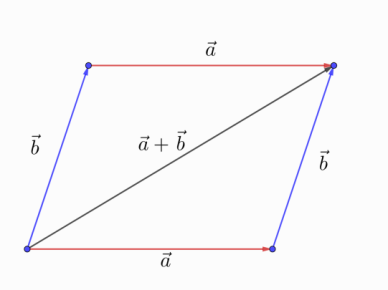
\includegraphics[width=0.4\textwidth]{images/pravilo_parallelogramma.png}
\end{center}

\begin{definition}
	\textit{Произведение вектора на число} $\overline{b} = \lambda\overline(a)$ $-$ вектор коллинеарный данному, а его модуль равен модулю данного вектора, умноженного на число. При этом
	\begin{enumerate}
		\item $\lambda = 0 \longrightarrow \overline{b} = \overline{0}$
		\item $\lambda < 0 \longrightarrow \overline{b}$ противоположно направлен $\overline{a}$
		\item $\lambda > 0 \longrightarrow \overline{b}$ сонаправлен $\overline{a}$
	\end{enumerate}
\end{definition}

\begin{definition}
	\textit{Разность векторов} определяется через операции сложения и умножения на число $\overline{a} - \overline{b} = \overline{a} + (-1)\overline{b}$.
\end{definition}

\textit{Свойства операций над векторами:}
\begin{enumerate}
	\item $\forall\overline{a},\overline{b}\tab\overline{a} + \overline{b} = \overline{b} + \overline{a}$
	\item $\forall\overline{a},\overline{b},\overline{c}\tab\overline{a} + (\overline{b} + \overline{c}) = (\overline{a} + \overline{b}) + \overline{c}$
	\item $\forall\overline{a}\tab\overline{a} + \overline{0} = \overline{a}$
	\item $\forall\overline{a}\tab\exists(-1)\overline{a} = -\overline{a}$ $-$ противоположный : $\overline{a} + (-\overline{a}) = \overline{0}$
	\item $\forall \alpha,\beta\in\R,\forall\overline{a}\tab(\alpha\beta)\overline{a}=\alpha(\beta\overline{a})$
	\item$\forall\overline{a}\tab1\cdot\overline{a}=\overline{a}$
	\item$\forall\alpha,\beta\in\R\tab(\alpha + \beta)\overline{a} = \alpha\overline{a}+\beta\overline{a}$
	\item$\forall\alpha\in\R,\forall\overline{a},\overline{b}\tab\alpha(\overline{a}+\overline{b})=\alpha\overline{a}+\alpha\overline{b}$
\end{enumerate}
\subsection{Линейная комбинация. Линейная зависимость и независимость}

\begin{definition}
	Если существует $\overline{a_1}$, ..., $\overline{a_n}$ и $\alpha_1$, ..., $\alpha_n$, то $\overline{b}=\alpha_1\overline{a_1}+...+\alpha_n\overline{a_n}$ $-$ $\textit{линейная комбинация}$. 
\end{definition}

Линейная комбинация называется $\textit{тривиальной}$, если все коэффициенты $\alpha_1=...=\alpha_n=0$, иначе $\textit{нетривиальной}$.

\begin{definition}
	Набор векторов $\overline{a_1}$, ..., $\overline{a_n}$ называют $\textit{линейно зависимым}$, если
	\begin{center}
		$\exists\alpha_1$, ..., $\alpha_n$ : $\alpha_1^2+...+\alpha_n^2 > 0$ : $\alpha_1\overline{a_1}+...+\alpha_n\overline{a_n} = \overline{0}$
	\end{center}
\end{definition}

\begin{definition}
	Набор векторов называется $\textit{линейно независимым}$, если только тривиальная комбинация дает нулевой вектор.
\end{definition}

\textit{Свойства:}

\begin{enumerate}
	\item если в наборе есть нулевой вектор, то этот набор линейно зависим
	\item если $\exists\overline{a_1}$, ..., $\overline{a_n}$ $-$ линейно зависимая комбинация, то $\forall\overline{b_1}$, ..., $\overline{b_m}$, то набор $\overline{a_1}$, ..., $\overline{a_n}, \overline{b_1}$, ..., $\overline{b_m}$ $-$ линейно зависмый
	\item если набор линейно независим, то его любой непустой поднабор тоже линейно независим
	\begin{proof}
		Пусть этот поднабор линейно независим, но тогда по свойству 2 весь набор линейно зависм $\longrightarrow$ противоречие.
	\end{proof}
\end{enumerate}

\begin{theorem}
	Пусть $\overline{x}$ $-$ линейная комбинация, т.е. $\overline{x}=\alpha_1\overline{a_1}+...+\alpha_n\overline{a_n}$. Тогда разложение $\overline{x}$ единсьвенное $\longleftrightarrow$ $\overline{a_1}$, ..., $\overline{a_n}$ $-$ линейно независмый набор.
\end{theorem}

\begin{proof}
	\tab
	$\longrightarrow$\\
	Пусть существует
	\begin{center}
		$\overline{x}=\alpha_1\overline{a_1}+...+\alpha_n\overline{a_n}\tab(1)$\\
		$\overline{x}=\beta_1\overline{a_1}+...+\beta_n\overline{a_n}\tab(2)$
	\end{center}
	Вычтем (1) из (2) $\longrightarrow$ существует $\alpha_i\neq\beta_i$ $\longrightarrow$ нетривиальная $\longrightarrow$ противоречие.
	
	$\tab\longleftarrow$\\
	Пусть $\overline{a_1}$, ..., $\overline{a_n}$ - линейно зависим $\longrightarrow$ $\exists$нетривиальная линейная комбинация $\gamma_1\overline{a_1}$, ..., $\gamma_n\overline{a_n} = \overline{0}$\\
	
	$\overline{x} = \overline{x} + \overline{0} = (\alpha_1 + \gamma_1)\overline{a_1}+...+(\alpha_n + \gamma_n)\overline{a_n}$ $\longrightarrow$ разложение не единственно $\longrightarrow$ противоречие.
\end{proof}

\begin{theorem}[Критерий линейной зависимости]
	Набор из k > 1 элементов линейно зависим $\longleftrightarrow$ существует вектор набора, равный линейной комбинации остальных.
\end{theorem}
\begin{proof}
	$\tab\longrightarrow$\\
	Предположим, что $\overline{a_1}$, ..., $\overline{a_k}$ $-$ линейно зависима, тогда $\exists\alpha_1$, ..., $\alpha_k$ :  $\alpha_1^2+...+\alpha_k^2$ > 0, $\alpha_1\overline{a_1}+...+\alpha_k\overline{a_k}=\overline{0}$.\\
	Пусть $\alpha_1\neq0$ $\longrightarrow$ $\overline{a_1} = -\frac{\alpha_2}{\alpha_1}\overline{a_2}-...-\frac{\alpha_k}{\alpha_1}\overline{a_2}$ $-$ вектор $\overline{a_1}$ раскладывается по остальным векторам.
	
	$\tab\longleftarrow$\\
	Пусть $\overline{a_1} = p_2\overline{a_2}+...+p_k\overline{a_k}$, тогда коэффициент при $\overline{a_1}$ = 1 $\longrightarrow$ $1\cdot\overline{a_1}+(-p_2)\overline{a_2}+...+(-p_k)\overline{a_k}=\overline{0}$ $-$ нетривиальная комбинация $\longrightarrow$ линейно зависимая.
\end{proof}

\begin{corollary}
	Рассмотрим следствия 1 - 3 без доказательства, т.к. они очевидны.\\
	\begin{enumerate}
		\item нетривиальная комбинация векторов линейно независимого набора всегда не равна $\overline{0}$
		\item система из одно вектора линейно зависима $\longleftrightarrow$ этот вектор нулевой
		\item система из двух векторов линейно зависима $\longleftrightarrow$ эти векторв коллинеарны
		\item система из трех векторов линейно зависима $\longleftrightarrow$ эти векторы компланарны
		\begin{proof}
			Пусть $\overline{a}, \overline{b}, \overline{c}$ $-$ компланарны.
			\begin{enumerate}
				\item Пусть $\overline{a}$ и $\overline{b}$ $-$ коллинеарны $\longrightarrow$ из следствия 3 они линейно зависимы, а значит весь набор линейно зависим.
				\item Пусть эти векторы неколлинеарны, тогда по правилу параллелограмма $\exists\alpha, \beta$ : $\alpha\overline{a}+\beta\overline{b}=\overline{c}$
			\end{enumerate}
		\end{proof}
		
		\item система из четырех и более векторов линейно зависима всегда
		\begin{proof} Пусть даны векторы $\overline{a}, \overline{b}, \overline{c}, \overline{d}$.
			\begin{enumerate}
				\item Если есть нулевой вектор, то набор линейно завсимый
				\item если все векторы ненулевые
				\begin{enumerate}
					\item Если $\overline{a}, \overline{b}, \overline{c}$ $-$ компланарны, то из следствия 4 вся система линейно зависима
					\item Если $\overline{a}, \overline{b}, \overline{c}$ $-$ некомпланарны достаточно доказать, что $\overline{d}$ является их линейной комбинацией.\\
					Для этого построим плоскость, проходящую через векторы Если $\overline{a}, \overline{b}$C. Проведем через $\overline{d}$ вектор, параллельный $\overline{c}$ $-$ $\overline{c_1}$.
					\begin{center}
						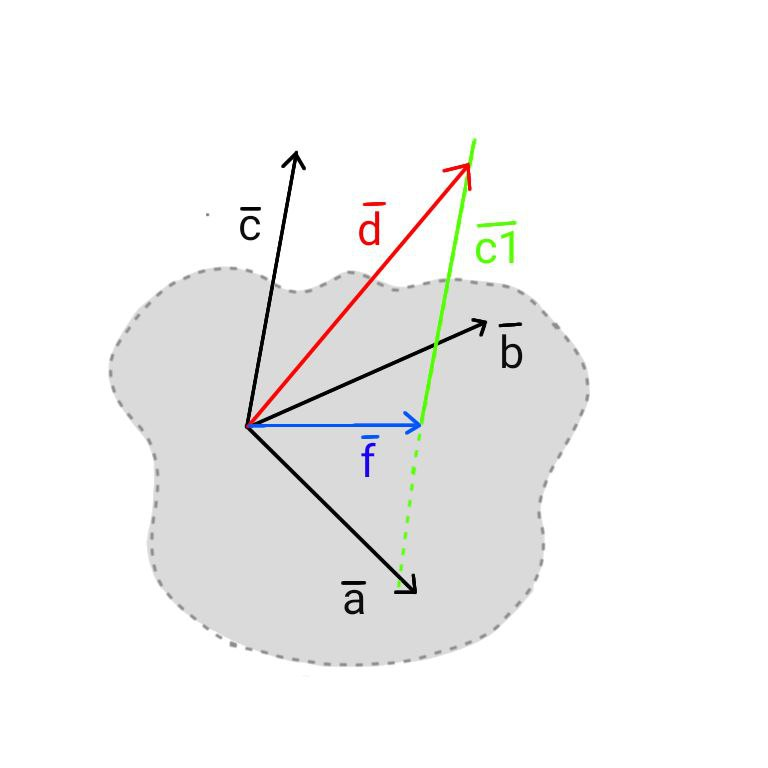
\includegraphics[width=0.4\textwidth]{images/5.jpeg}
					\end{center}
				\end{enumerate}
				$\overline{f}$ $-$ вектор к точке пересечения $\overline{c_1}$ с плоскостью. Т.к. Если $\overline{a}$ и $\overline{b}$ неколлинеарные, $\overline{f}$ можно разложить по ним:\\
				$\begin{cases}
					\overline{f} = \alpha\overline{a}+\beta\overline{b}\\
					\overline{c_1}=\gamma\overline{c}\\
				\end{cases}$ $\longrightarrow$ $\overline{d}=\overline{f}+\overline{c_1}= \alpha\overline{a}+\beta\overline{b}+\gamma\overline{c}$, значит $\overline{d}$ раскладывается по остальным векторам и система линейно зависимая.
			\end{enumerate}
		\end{proof}
		
	\end{enumerate}
\end{corollary}











\section{Базис векторного пространства. Системы координат.}

\subsection{Пространства}

\begin{definition}
	Множество назовем $\textit{замкнутым}$ относительно операции, если результат применения этой операции принадлежит этому множеству.
\end{definition}

\begin{definition}
	Непустое множество, замкнутое относительно линейных операций (сложение и умножение на число), назовем $\textit{векторным пространством}$.
\end{definition}

Если одно векторное пространство является подмножеством другого, будем называть его $\textit{подпространством}$.

Само множество является своим подмножеством $\longrightarrow$ пространство является своим подпространством.


\subsection{Базис в векторном пространстве}

\begin{definition}
	$\textit{Базис в векторном пространстве}$ $-$ упорядоченный линейно независимый набор векторов, такой, что любой вектор пространства раскладывается по этим векторам.
\end{definition}

В нулевом пространстве базиса нет.

В одномерном пространстве базис $-$ любой ненулевой вектор.

В двумерном пространстве базис $-$ упорядоченная пара неколлинеарных векторов.

В трехмерном пространстве базис $-$ упорядоченная тройка некомпланарных векторов.\\

Любой вектор раскладывается по векторам базиса, и это разложение единственно.\\

Пусть существует базис ($\overline{e_1}, \overline{e_2}, \overline{e_3}$), такой что любой вектор в этом базисе $\overline{a} = x_1\overline{e_1} + x_2\overline{e_2} + x_3\overline{e_3}$. Тогда коэффициенты разложения $x_1$, $x_2$, $x_3$ определяются единственным образом и называются $\textit{координатами}$.\\

Пусть в этом же базисе существуют вектора $\overline{a}(a_1, a_2, a_3), \overline{b}(b_1, b_2, b_3), \overline{c}(c_1, c_2, c_3)$. Узнаем, является ли этот набор линейно зависимым. Для этого необходимо узнать, существует ли их нетривиальная комбинация:

\begin{center}
	$\alpha\overline{a} + \beta\overline{b} + \gamma\overline{c} = \overline{0}\tab\longleftrightarrow$\\
	
	$\alpha
	\begin{pmatrix*}
		a_1\\
		a_2\\
		a_3\\
	\end{pmatrix*} + \beta
	\begin{pmatrix*}
		b_1\\
		b_2\\
		b_3\\
	\end{pmatrix*} + \gamma
	\begin{pmatrix*}
		c_1\\
		c_2\\
		c_3\\
	\end{pmatrix*} = 
	\begin{pmatrix*}
		0\\
		0\\
		0\\
	\end{pmatrix*}$
\end{center} $\longrightarrow$ по теореме Крамера система имеет единственное решение, отличное от тривиальной комбинации, при
\begin{center}
	det = 
	$\begin{vmatrix}
		a_1 & b_1 & c_1\\
		a_2 & b_2 & c_2\\
		a_3 & b_3 & c_3\\
	\end{vmatrix} \longrightarrow$ если det = 0, система линейно зависима, иначе $-$ линейно независима.
	
\end{center}

Аналогично для плоскости.

\subsection{Декартова и некоторые другие системы координат}

\begin{wrapfigure}{l}{0.4\textwidth}
	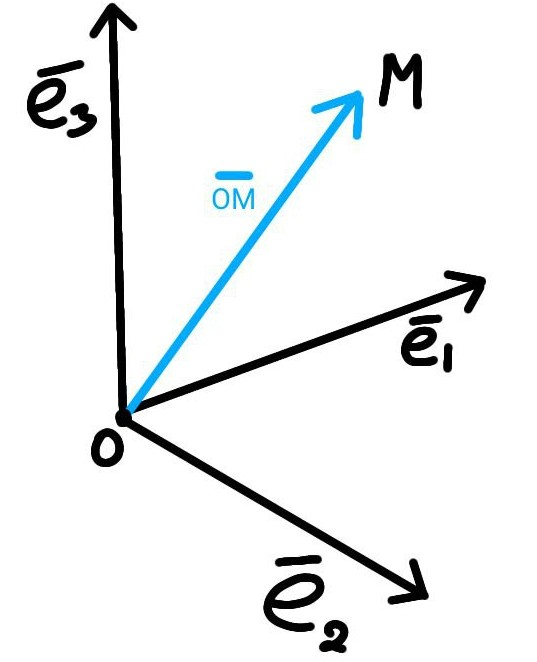
\includegraphics[width=0.5\linewidth]{images/дск.jpeg}
\end{wrapfigure}

\begin{definition}
	\textit{Декартова система координат} $-$ совокупность точки и базиса.
\end{definition}

\tab\\ \tab\\
O $-$ начало координат\\
$\overline{e_1}, \overline{e_2}, \overline{e_3}$ $-$ базис\\
$\overline{OM}$ = $x_1\overline{e_1} + x_2\overline{e_2} + x_3\overline{e_3}$ $\longrightarrow$ $x_1, x_2, x_3$ $-$ координаты.

\tab\\ \tab\\ \tab\\ \tab\\ \tab\\

\textbf{Медианный вектор}\\

\begin{wrapfigure}{r}{0.4\textwidth}
	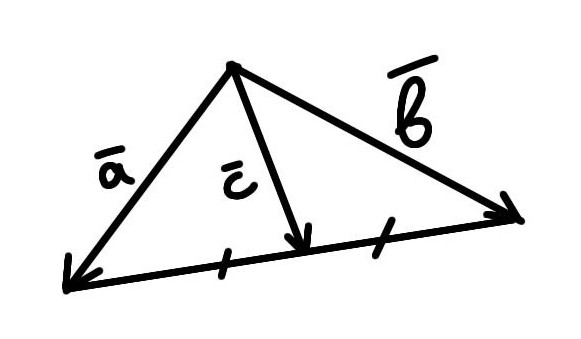
\includegraphics[width=0.8\linewidth]{images/медианныйвектор.jpeg}
\end{wrapfigure}

Пусть $\overline{a}, \overline{b}$ $-$ образующие векторы, $\overline{c}$ $-$ медианный. Тогда $\overline{c}$ = $\frac{\overline{a} + \overline{b}}{2}$.\\

Аналогично можно найти координаты середины отрезка, с концами в координатах ($a_1, a_2, a_3$) и ($b_1, b_2, b_3$), M = ($\frac{a_1 - b_1}{2}, \frac{a_2 - b_2}{2}, \frac{a_3 - b_3}{2}$)

\tab\\ \tab\\

\textbf{Вектор, коллинеарный биссектрисе угла}

\begin{wrapfigure}{l}{0.4\textwidth}
	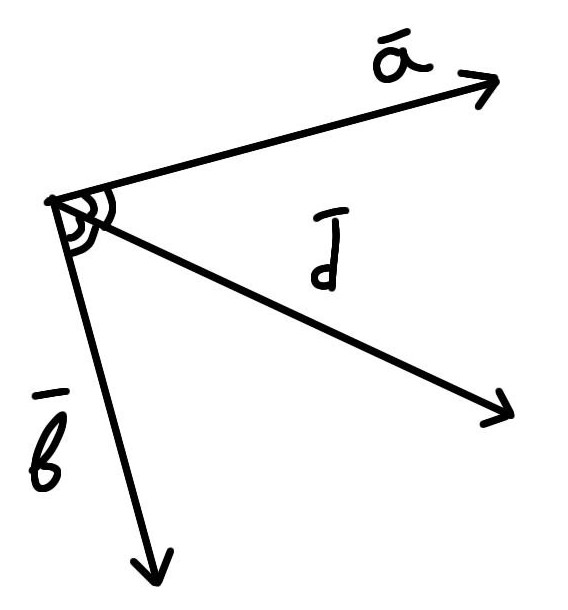
\includegraphics[width=0.6\linewidth]{images/биссектриса.jpeg}
\end{wrapfigure}

\tab\\ \tab\\

Пусть $\overline{d}$ $-$ вектор, коллинеарный биссектрисе угла, построенного на векторах $\overline{a}$ и $\overline{b}$.\\
 
$\overline{d}$ = $\frac{\overline{a}}{|\overline{a}|} + \frac{\overline{b}}{|\overline{b}|}$

\tab\\ \tab\\ \tab\\ \tab\\
\textbf{Вектор, который делит прямую в соотношении m:n}

\begin{wrapfigure}{r}{0.4\textwidth}
	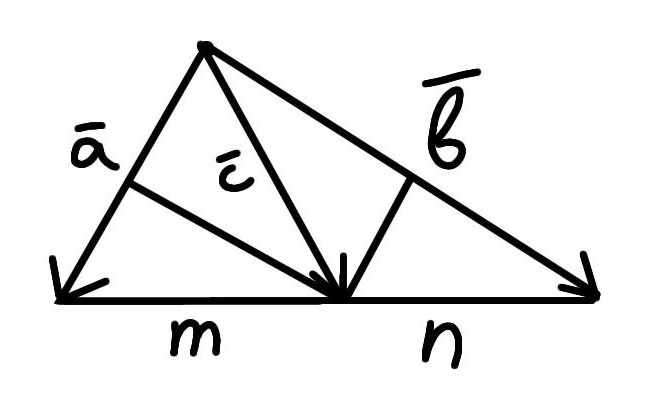
\includegraphics[width=0.6\linewidth]{images/соотношение.jpeg}
\end{wrapfigure}

\tab\\

$\overline{c}$ = $\frac{n}{m + n}\overline{a} + \frac{m}{m + n}\overline{b}$

\tab\\ \tab\\ \tab\\ \tab\\

\begin{definition}
	Если базисные векторы попарно ортогональны, то базис \textit{ортогональный}.
\end{definition}

\begin{definition}
	Если базисные векторы попарно ортогональны, а их длины равны 1, то базис \textit{ортонормированный} (ОНБ).
\end{definition}

\begin{definition}
	Система координат с ОНБ $-$ \textit{декартова прямоугольная система координат}.
\end{definition}

\textbf{Полярная система координат}\\
\begin{wrapfigure}{l}{0.4\textwidth}
	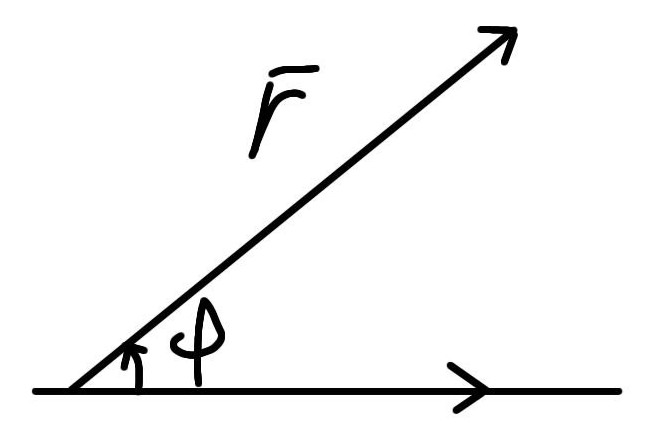
\includegraphics[width=0.6\linewidth]{images/полярнаяск.jpeg}
\end{wrapfigure}

Координаты задаются длиной радиус-вектора $\overline{r}$ и полярным углом $\phi$.\\

$\overline{r}(|\overline{r}|, \phi)$

\tab\\ \tab\\ \tab\\

\textbf{Цилиндрическая система координат}\\
\begin{wrapfigure}{l}{0.4\textwidth}
	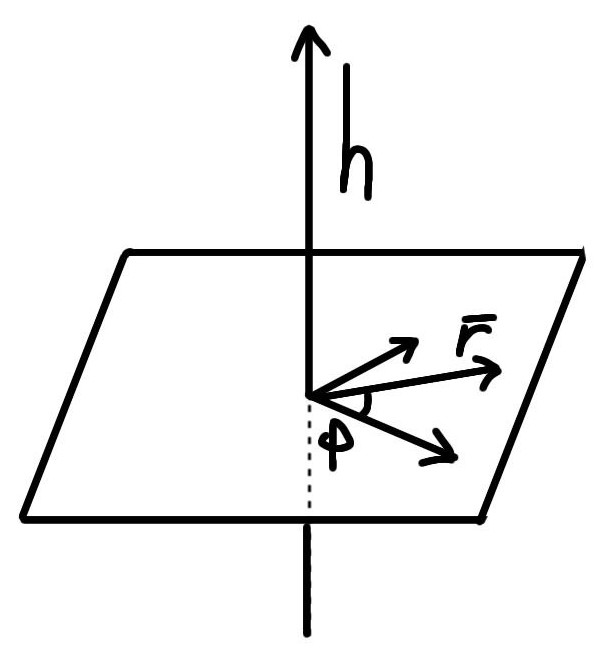
\includegraphics[width=0.6\linewidth]{images/цилиндрическаяск.jpeg}
\end{wrapfigure}

Координаты задаются длиной радиус-вектора $\overline{r}$, полярным углом $\phi$ и смещением относительно оси z.\\

$\overline{r}(|\overline{r}|, \phi, h)$

\tab\\ \tab\\ \tab\\ \tab\\ \tab\\ \tab\\
\textbf{Сферическая система координат}\\
\begin{wrapfigure}{l}{0.4\textwidth}
	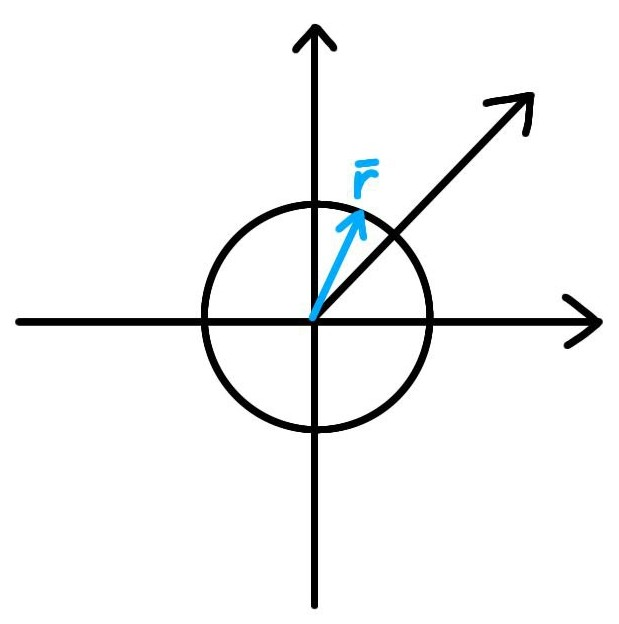
\includegraphics[width=0.5\linewidth]{images/сферическая.jpeg}
\end{wrapfigure}

Координаты задаются длиной радиус-вектора $\overline{r}$, азимутальным углом $\phi\in[0, 2\pi]$ и зенитным углом $\theta\in[-\frac{\pi}{2}, \frac{\pi}{2}]$.\\

$\overline{r}(|\overline{r}|, \theta, \phi)$
\tab\\ \tab\\ \tab\\ \tab\\ \tab\\
\newpage

\subsection{Переход в новую систему координат}

Пусть имеются две системы координат и вектор $\overline{a}$:\\
\tab\\
$\tab$($\overline{e_1}, \overline{e_2}, \overline{e_3})$ $-$ "старая" система координат, $\overline{a}$(x, y, z)\\
$\tab$($\overline{e_1'}, \overline{e_2'}, \overline{e_3'})$ $-$ "новая" система координат, $\overline{a}$(x', y', z')\\

Тогда базисные векторы новой системы координат выражаются следующим образом:\\
\tab\\
$\overline{e_1'}$ = $a_{11}\overline{e_1} + a_{21}\overline{e_2} + a_{31}\overline{e_3}$\\
$\overline{e_2'}$ = $a_{12}\overline{e_1} + a_{22}\overline{e_2} + a_{32}\overline{e_3}$\\
$\overline{e_3'}$ = $a_{13}\overline{e_1} + a_{23}\overline{e_2} + a_{33}\overline{e_3}$\\

В новой системе координат $\overline{a}$ = $x'\overline{e_1'} + y'\overline{e_2'} + z'\overline{e_3'}$ = $x'(a_{11}\overline{e_1} + a_{21}\overline{e_2} + a_{31}\overline{e_3}) + y'(a_{12}\overline{e_1} + a_{22}\overline{e_2} + a_{32}\overline{e_3}) + z'(a_{13}\overline{e_1} + a_{23}\overline{e_2} + a_{33}\overline{e_3})$ = $\overline{e_1}(a_{11}x' + a_{12}y' + a_{13}z') + \overline{e_2}(a_{21}x' + a_{22}y' + a_{23}z') + \overline{e_3}(a_{31}x' + a_{32}y' + a_{33}z')\tab\longrightarrow$\\
\tab\\
x = $a_{11}x' + a_{12}y' + a_{13}z'$\\
y = $a_{21}x' + a_{22}y' + a_{23}z'$\\
z = $a_{31}x' + a_{32}y' + a_{33}z'$\\

\begin{definition}
	\textit{Матрица перехода} от базиса e к базису e' имеет вид\\
	\begin{center}
		S =
		$\begin{pmatrix}
			a_{11} & a_{12} & a_{13}\\
			a_{21} & a_{22} & a_{23}\\
			a_{31} & a_{32} & a_{33}\\
		\end{pmatrix}$
	\end{center} 
\end{definition}

Столбцами S являются координаты новых базисных векторов в старом базисе.\\

\begin{center}
	$\begin{pmatrix*}
		x\\
		y\\
		z\\
	\end{pmatrix*}$ = S
	$\begin{pmatrix*}
		x'\\
		y'\\
		z'\\
	\end{pmatrix*}$, $\tab$ ($\overline{e_1'}, \overline{e_2'}, \overline{e_3'}$) = ($\overline{e_1}, \overline{e_2}, \overline{e_3}$)S, $\tab$ e' = eS
\end{center}

\textbf{Основное свойство матрицы перехода:} по теореме о линейной независимости, det S $\neq$ 0.

Рассмотрим старое начало координат О и новое О'. Тогда вектор, соединяющий их\\

\begin{wrapfigure}{l}{0.4\textwidth}
	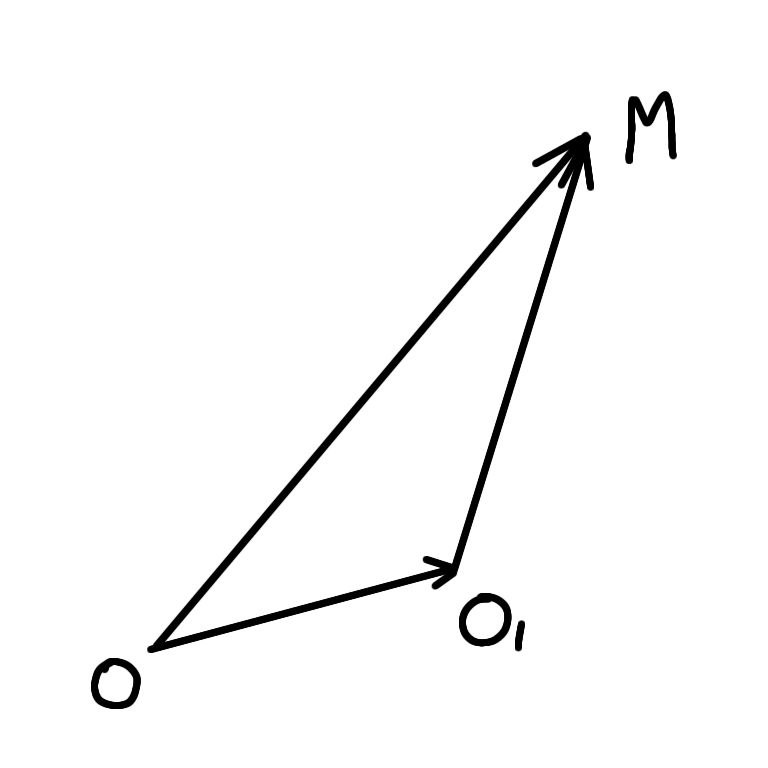
\includegraphics[width=0.6\linewidth]{images/переход1.jpeg}
\end{wrapfigure}

$\overline{OO'}$ = $\beta_1\overline{e_1} + \beta_2\overline{e_2} + \beta_3\overline{e_3}$ \\

Пусть существует произвольная точка М, такая что $\overline{OM}$ = $\overline{OO'} + \overline{O'M}$. Тогда ее координаты\\

x = $a_{11}x' + a_{12}y' + a_{13}z' + \beta_1$\\
y = $a_{21}x' + a_{22}y' + a_{23}z' + \beta_2$\\
z = $a_{31}x' + a_{32}y' + a_{33}z' + \beta_3$\\












\section{Скалярное, векторное и смешанное произведения}

\subsection{Скалярное произведение}

\begin{definition}
    \textit{Скалярное произведение} c = $(\overline{a}, \overline{b})$ определяется по следующим правилам:

    \begin{enumerate}
        \item Если $\overline{a}$ = 0 или $\overline{b}$ = 0, то с = 0
        \item Если $\overline{a}$ $\neq$ 0 и $\overline{b}$ $\neq$ 0, то с = $|\overline{a}|\cdot|\overline|b|\cdot cos(\overline{a}, \overline{b})$
    \end{enumerate}
\end{definition}

\textit{Свойства скалярного произведения:}

\begin{enumerate}
    \item ($\overline{a}, \overline{b}$) = 0 $\longleftrightarrow$
    $\begin{gathered}
        \overline{a} = \overline{0}\\
        \overline{b} = \overline{0}\\
        \overline{a} \perp \overline{b}\\
    \end{gathered}$
    \item $\forall\overline{a}, \overline{b}\hookrightarrow(\overline{a}, \overline{b}) = (\overline{b}, \overline{a})$
    \item $\forall\overline{a}$    $(\overline{a}, \overline{a}) = |\overline{a}|^2\geq0$ $-$ скалярный квадрат
    \item $\forall\overline{a}$    $(\overline{a}, \overline{a}) = 0 \longleftrightarrow \overline{a} = \overline{0}$
\end{enumerate}

\begin{lemma}
    Пусть $\overline{a}$ $-$ фиксированный вектор, тогда $\forall\overline{x}$
    \begin{center}
        ($\overline{a}, \overline{x}$) = 0 $\longrightarrow \overline{a} = \overline{0}$
    \end{center}
\end{lemma}

Для векторов ортонормированного базиса:
\begin{center}
    ($\overline{e_i}, \overline{e_j}$) = 
    $\begin{cases}
        0, i \neq  j\\
        1, i = j\\
    \end{cases}$
\end{center}

Пусть базис $\overline{e_1}, \overline{e_2}, \overline{e_3}$ $-$ ортогональный, тогда координаты вектора $\overline{a}$ находятся по формулам:

\begin{center}
    $a_1$ = $\dfrac{(\overline{a}, \overline{e_1})}{|\overline{e_1}|^2 }$, $a_2$ = $\dfrac{(\overline{a}, \overline{e_2})}{|\overline{e_2}|^2 }$, $a_3$ = $\dfrac{(\overline{a}, \overline{e_3})}{|\overline{e_3}|^2 }$
\end{center}

В ортонормированном базисе:

\begin{center}
    $\overline{a}$ = $(\overline{a}, \overline{e_1})\overline{e_1} + (\overline{a}, \overline{e_2})\overline{e_2} + (\overline{a}, \overline{e_3})\overline{e_3}$
\end{center}

\begin{theorem}
    \textit{Свойство линейности скалярного произведения:}
    \begin{center}
        $\forall\alpha,\beta\in\R, \forall\overline{a}, \overline{b}, \overline{c}$\\
        $(\alpha\overline{a} + \beta\overline{b}, \overline{c})$ = $\alpha(\overline{a}, \overline{c}) + \beta(\overline{b}, \overline{c})\tab(1)$\\
        $(\overline{c}, \alpha\overline{a} + \beta\overline{b})$ = $\alpha(\overline{c}, \overline{a}) + \beta(\overline{c}, \overline{b})\tab(2)$
    \end{center}
\end{theorem}
\begin{proof}
    (2) следует из (1), поэтому докажем только (1)\\

    Рассмотрим случаи.
    
    \begin{enumerate}
        \item $\overline{c} = \overline{0} \longrightarrow$ утверждение верно
        \item $\overline{c} \neq \overline{0} \longrightarrow$ Рассмотрим ортогональный базис, в котороом $\overline{c}$ = $\overline{e_1}$. Докажем равенство, эквивалентное (1):
        \[
        \dfrac{(\alpha\overline{a} + \beta\overline{b}, \overline{c})}{|\overline{c}|^2} = \dfrac{\alpha(\overline{a}, \overline{c})}{|\overline{c}|^2} + \dfrac{\beta(\overline{b}, \overline{c})}{|\overline{c}|^2}
        \]
        Слева первая координата вектора $\alpha\overline{a} + \beta\overline{b}$ в базисе.\\
        Справа также первая координата ветора $\alpha\overline{a} + \beta\overline{b}$ в базисе $\longrightarrow$ ч.т.д.
    \end{enumerate}
\end{proof}

\begin{corollary}
    Если в каком-то базисе у векторов равные координаты, то данные векторы равны в любом базисе.
\end{corollary}

Пусть имеется двумерный базис $\overline{e_1}$, $\overline{e_2}$, $\overline{a}(a_1, a_2)$, $\overline{b}(b_1, b_2)$, тогда
\[
(\overline{a}, \overline{b}) = (a_1\overline{e_1} + a_2\overline{e_2}, b_1\overline{e_1} + b_2\overline{e_2}) = a_1 b_1(\overline{e_1}, \overline{e_1}) + a_1 b_2(\overline{e_1}, \overline{e_2}) + a_2 b_1(\overline{e_2}, \overline{e_1}) + a_2 b_2(\overline{e_2}, \overline{e_2})
\]
Аналогично для трехмерного пространства.\\

\begin{theorem}
    Рассмотрим базис $\overline{e_1}, \overline{e_2}, \overline{e_3}$. Тройка $\overline{e_1}*, \overline{e_2}*, \overline{e_3}*$ определяется однозначно и образует базис, если она является $\textit{биортогональным (взаимным)}$ базисом, т.е. выполняется следующее условие
    \[
    (\overline{e_i}, \overline{e_j}*) = 
    \begin{cases}
        0, i \neq  j\\
        1, i = j\\
    \end{cases}
    \]
\end{theorem}

\begin{proof}
    \tab\\
    \begin{enumerate}
        \item Определяется однозначно.\\
            
        $\overline{e_1}* \perp \overline{e_2}, \overline{e_3}$\\
        $\overline{e_1}$ направлен в то же полупространство, что и $\overline{e_1}*$ $\longrightarrow$ $(\overline{e_1}*, \overline{e_1})$ определено однозначно $\longrightarrow$ |$\overline{e_1}*$| определено однозначно.\\
        Аналогично для $\overline{e_2}*, \overline{e_3}*$ $\longrightarrow$ ч.т.д.

        \item Образует базис.\\

        Пусть $\overline{x}$ раскладывается по $\overline{e_1}*, \overline{e_2}*, \overline{e_3}*$ $\longrightarrow$ $\overline{x} = \alpha_1\overline{e_1}* + \alpha_2\overline{e_2}* + \alpha_3\overline{e_3}*$\\
        Скаляроне умножение на $\overline{e_1}$: ($\overline{x}, \overline{e_1}$) = $\alpha_1(\overline{e_1}, \overline{e_1}*) + \alpha_2(\overline{e_2}, \overline{e_2}*) + \alpha_3(\overline{e_3}, \overline{e_3}*)$, что по определению равно $\alpha_1$ $\longrightarrow$ $\alpha_1$ определяется однозначно.

        Аналогично для $\alpha_2$ и $\alpha_3$, значит, по теореме о линейной независимости, ч.т.д.
    \end{enumerate}
\end{proof}

\begin{corollary}
    \tab\\
    \begin{enumerate}
        \item Для $\overline{e_1}*, \overline{e_2}*, \overline{e_3}*$ базис $\overline{e_1}, \overline{e_2}, \overline{e_3}$ $-$ биортогональный.
        \item Ортонормированный базис взаимен самому себе.
        \item Пусть известны координаты $\overline{a}(a_1, a_2, a_3)$ в базисе $\overline{e_1}, \overline{e_2}, \overline{e_3}$ и $\overline{b}(b_1, b_2, b_3)$ в базисе $\overline{e_1}*, \overline{e_2}*, \overline{e_3}*$ $\longrightarrow$
        \[
        (\overline{a}, \overline{b}) = \alpha_1 \beta_1* + \alpha_2 \beta_2* + \alpha_3 \beta_3*
        \]
    \end{enumerate}
\end{corollary}

\textbf{Нахождение проекции вектора}\\
\begin{wrapfigure}{l}{0.4\textwidth}
	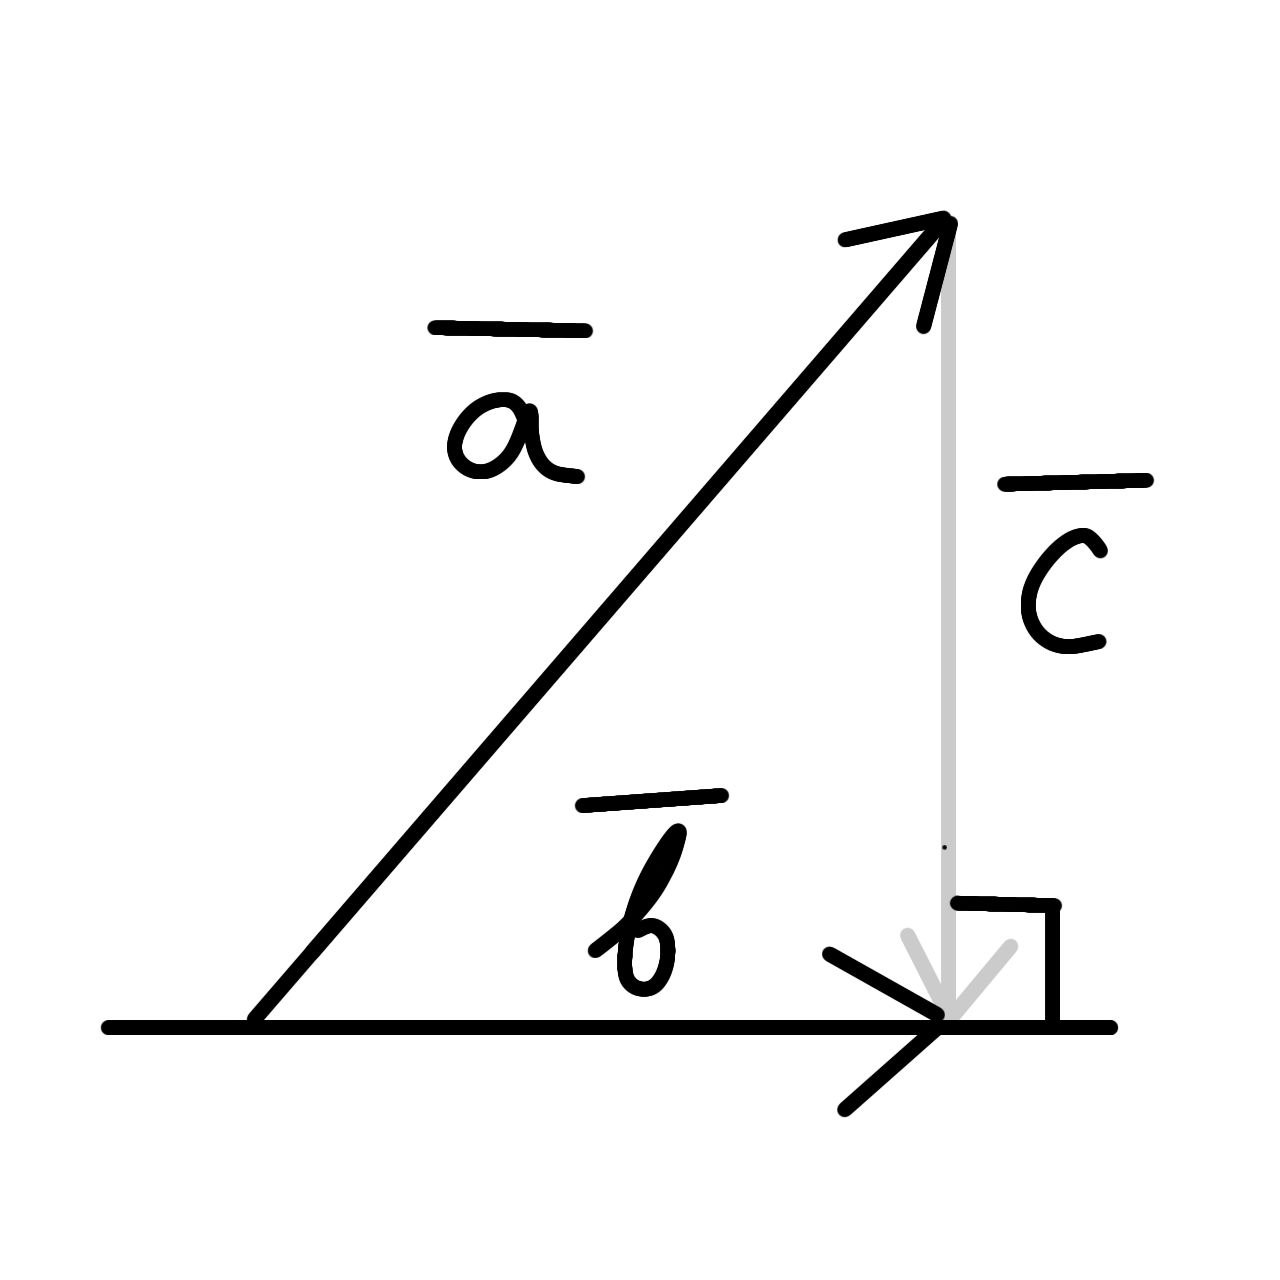
\includegraphics[width=0.84\linewidth]{images/проекция.jpeg}
\end{wrapfigure}

Пусть $\overline{a}$ $-$ вектор, который проецируем, $\overline{b}$ $-$ вектор, на который проецируем, $\overline{c}$ $-$ ортогональная составляющая.

\[
\text{Пр}_{\overline{b}}^{\overline{a}} = |\overline{a}| \cdot cos\thinspace\phi \cdot \dfrac{\overline{b}}{|\overline{b}|} = \dfrac{(\overline{a}, \overline{b})}{|\overline{b}|^2}\overline{b},
\]

где $\dfrac{(\overline{a}, \overline{b})}{|\overline{b}|^2}$ $-$ численное значение проекции

\tab\\ \tab\\ \tab\\ \tab\\

\subsection{Векторное произведение}

\begin{definition}
    Упорядоченную тройку векторов $\overline{a}, \overline{b}, \overline{c}$ назовем $\textit{правой}$, если при рассмотрении из полупространства, в которое направлен вектор $\overline{c}$ крачайший поворот от $\overline{a}$  к $\overline{b}$ направлен против часовой стрелки.\\

    Иначе $\overline{a}, \overline{b}, \overline{c}$ $-$ $\textit{левая}$ тройка.
\end{definition}

Если $\overline{a}, \overline{b}, \overline{c}$ $-$ правая, то $\overline{c}, \overline{a}, \overline{b}$ $-$ правая, а $\overline{b}, \overline{a}, \overline{c}$ $-$ левая.

\begin{definition}
    $\textit{Векторное произведение}$ $\overline{a}$ и $\overline{b}$  $\overline{c} = [\overline{a}, \overline{b}]$ определяется следующим образом:
    \begin{enumerate}
        \item если $\overline{a}$ и $\overline{b}$ $-$ коллинеарные (включая $\overline{0}$), то $\overline{c} = 0$
        \item если $\overline{a}$ и $\overline{b}$ $-$ неколлинеарные, то 
        \begin{itemize}
            \item $|\overline{c}| = |\overline{a}|\cdot|\overline{b}|\cdot sin(\overline{a}, \overline{b})$
            \item $\overline{a}\perp\overline{c}$, $\overline{b}\perp\overline{c}$
            \item $\overline{a}, \overline{b}, \overline{c}$ $-$ правая тройка
        \end{itemize}
    \end{enumerate}
\end{definition}

\textit{Свойства векторного произведения:}

\begin{enumerate}
    \item $[\overline{a}, \overline{b}]$ = $\overline{0}$ $\longleftrightarrow$ $\overline{a}$ и $\overline{b}$ $-$ коллинеарные
    \item $\forall\overline{a}, \overline{b}$ $[\overline{a}, \overline{b}] = - [\overline{b}, \overline{a}]$
    \item $|[\overline{a}, \overline{b}]|$ $-$ площадь параллелограмма, построенного на векторах $\overline{a}, \overline{b}$
    \item Свойство линейности векторного произведени:
    \[
    \forall\alpha, \beta \in \R\tab\forall\overline{a}, \overline{b}, \overline{c}\hookrightarrow[\alpha\overline{a} + \beta\overline{b}, \overline{c}] = \alpha[\overline{a}, \overline{c}] + \beta[\overline{b}, \overline{c}]
    \]
\end{enumerate}

Пусть известны базис $\overline{e_1}, \overline{e_2}, \overline{e_3}$, $\overline{a}(a_1, a_2, a_3)$, $\overline{b}(b_1, b_2, b_3)$ $\longrightarrow$ 

\begin{center}
    $[\overline{a}, \overline{b}]$ = $[a_1\overline{e_1} + a_2\overline{e_2} + a_3\overline{e_3}, b_1\overline{e_1} + b_2\overline{e_2} + b_3\overline{e_3}]$ = $\sum a_i b_j [\overline{e_i}, \overline{e_j}]$ = $[\overline{e_1}, \overline{e_2}](a_1 b_2 - a_2 b_1) + [\overline{e_2}, \overline{e_3}](a_2 b_3 - a_3 b_2) + [\overline{e_3}, \overline{e_1}](a_3 b_1 - a_1 b_3)$ = 
    $\begin{vmatrix}
        [\overline{e_2}, \overline{e_3}] & [\overline{e_3}, \overline{e_1}] & [\overline{e_1}, \overline{e_2}]\\
        a_1 & a_2 & a_3\\
        b_1 & b_2 & b_3\\
    \end{vmatrix}$
\end{center}

В правом ОНБ:
\[
    [\overline{a}, \overline{b}] = 
    \begin{vmatrix}
        \overline{e_1} & \overline{e_2} & \overline{e_3}\\
        a_1 & a_2 & a_3\\
        b_1 & b_2 & b_3\\
    \end{vmatrix}
\]
\subsection{Смешанное произведение}

\begin{definition}
    \textit{Смешанное произведение} векторов $\overline{a}, \overline{b}, \overline{c}$ определяется как 
    \[
    (\overline{a}, \overline{b}, \overline{c}) = ([\overline{a}, \overline{b}], \overline{c})
    \]
\end{definition}

\begin{theorem}
    Смешенное произведение равно объему ориентированного параллелепипеда, построенного на векторах $\overline{a}, \overline{b}, \overline{c}$
\end{theorem}

\begin{proof}
    \tab\\
    \begin{enumerate}
        \item $\overline{a}, \overline{b}$ $-$ коллинеарны $\longrightarrow$ 
        $\begin{cases}
            (\overline{a}, \overline{b}, \overline{c}) = 0\\
            V = 0\\
        \end{cases}$
        \item $\overline{a}, \overline{b}$ $-$ неколлинеарны
        \begin{itemize}
            \item $\overline{a}, \overline{b}, \overline{c}$ $-$ компланарны $\longrightarrow$
            $\begin{cases}
                (\overline{a}, \overline{b}, \overline{c}) = 0\\
                V = 0\\
            \end{cases}$
            \item $\overline{a}, \overline{b}, \overline{c}$ $-$ некомпланарны $\longrightarrow$
            \[
            V = S_{\text{осн}}\cdot h = |[\overline{a}, \overline{b}]|\cdot|\overline{c}|\cdot|cos\thinspace\phi| = |(\overline{a}, \overline{b}, \overline{c})|
            \]
        \end{itemize}
    \end{enumerate}
\end{proof}

\textit{Свойства смешанного произведения:}

\begin{enumerate}
    \item $(\overline{a}, \overline{b}, \overline{c})$ = $(\overline{b}, \overline{c}, \overline{a})$ = $(\overline{c}, \overline{a}, \overline{b})$ = -$(\overline{a}, \overline{c}, \overline{b})$ = -$(\overline{b}, \overline{a}, \overline{c})$ = -$(\overline{c}, \overline{b}, \overline{a})$
    \begin{corollary}
        $([\overline{a}, \overline{b}], \overline{c})$ = $(\overline{a}, [\overline{b}, \overline{c}])$
    \end{corollary}
    \item Линейность смешанного произведения:
    \[
    \forall\alpha_1, \alpha_2\tab\forall\overline{a_1}, \overline{a_2}, \overline{b}, \overline{c}\hookrightarrow (\alpha_1\overline{a_1} + \alpha_2\overline{a_2}, \overline{b}, \overline{c}) = \alpha_1(\overline{a_1}, \overline{b}, \overline{c}) + \alpha_2(\overline{a_2}, \overline{b}, \overline{c})
    \]
\end{enumerate}

\begin{theorem}
    \[
    [\overline{a}, \overline{b}], [\overline{b}, \overline{c}], [\overline{c}, \overline{a}] - \text{линейно независимые} \longleftrightarrow \overline{a}, \overline{b}, \overline{c} - \text{линейно независимые}
    \]
\end{theorem}
\begin{proof}
    \tab\\
    \begin{enumerate}
        \item $\overline{a}, \overline{b}, \overline{c}$ - компланарные $\longrightarrow$ векторные произведения или равны $\overline{0}$, или перпендикулярны векторам $\longrightarrow$ линейно зависимые
        \item $\overline{a}, \overline{b}, \overline{c}$ - некомпланарные $\longrightarrow$ $\exists \alpha,\beta,\gamma$ :
        \[
        \alpha[\overline{a}, \overline{b}] + \beta[\overline{b}, \overline{c}] + \gamma[\overline{c}, \overline{a}] = \overline{0}
        \]
        Скалярно домножим на $\overline{a}$ и получим
        \[
        0 + \beta(\overline{a}, \overline{b}, \overline{c}) + 0 = 0
        \]
        $\overline{a}, \overline{b}, \overline{c}$ $-$ некомпланарны $\longrightarrow$ $(\overline{a}, \overline{b}, \overline{c})\neq 0$ $\longrightarrow$ $\beta$ = 0, аналогично для $\alpha$ и $\gamma$ $\longrightarrow$ $\alpha=\beta=\gamma=0$ $-$ тривиальная комбинация $\longrightarrow$ $[\overline{a}, \overline{b}], [\overline{b}, \overline{c}], [\overline{c}, \overline{a}]$ $-$ линейно независимые
        
    \end{enumerate}
\end{proof}

\begin{corollary}
    Попарные векторные произведения линейно независимых векторов образуют базис.
\end{corollary}

\underline{\textbf{Задача.}} C помощью смешанного произведения определить, является ли тройка линейно зависимой.\\

В базисе $\overline{e_1}, \overline{e_2}, \overline{e_3}$ заданы векторы $\overline{a}(a_1, a_2, a_3), \overline{b}(b_1, b_2, b_3), \overline{c}(c_1, c_2, c_3)$ $\longrightarrow$

\begin{center}
    $(\overline{a}, \overline{b}, \overline{c})$ = $(\overline{a}, [\overline{b}, \overline{c}])$ = $(a_1\overline{e_1} + a_2\overline{e_2} + a_3\overline{e_3}$, $[\overline{e_1}, \overline{e_2}](b_1 c_2 - b_2 c_1) + [\overline{e_2}, \overline{e_3}](b_2 c_3 - b_3 c_2) + [\overline{e_3}, \overline{e_1}](b_3 c_1 - b_1 c_3))$ = 
        $\begin{vmatrix}
            [\overline{e_2}, \overline{e_3}] & [\overline{e_3}, \overline{e_1}] & [\overline{e_1}, \overline{e_2}]\\
            b_1 & b_2 & b_3\\
            c_1 & c_2 & c_3\\
        \end{vmatrix}(\overline{e_1}, \overline{e_2}, \overline{e_3})$
\end{center}

В правом ОНБ ($\overline{e_1}, \overline{e_2}, \overline{e_3}$) = 1

\begin{enumerate}
    \item $\overline{a}, \overline{b}, \overline{c}$ $-$ линейно зависимые в любом базисе $\longleftrightarrow$ \\
    $(\overline{a}, \overline{b}, \overline{c})$ = 
    $\begin{vmatrix}
        [\overline{e_2}, \overline{e_3}] & [\overline{e_3}, \overline{e_1}] & [\overline{e_1}, \overline{e_2}]\\
        b_1 & b_2 & b_3\\
        c_1 & c_2 & c_3\\
    \end{vmatrix}(\overline{e_1}, \overline{e_2}, \overline{e_3})$ $\neq$ 0

    \item $\overline{a}, \overline{b}$ $-$ коллинеарные, а значит, линейно зависимые для любого базиса $\longleftrightarrow$ [$\overline{a}, \overline{b}$] = 0 $\longleftrightarrow$
    $\begin{vmatrix}
        a_1 & a_2\\
        b_1 & b_2\\
    \end{vmatrix}$ = 
    $\begin{vmatrix}
        a_1 & a_3\\
        b_1 & b_3\\
    \end{vmatrix}$ =
    $\begin{vmatrix}
        a_2 & a_3\\
        b_2 & b_3\\
    \end{vmatrix}$ = 0
\end{enumerate}
\underline{\textbf{Некоторые полезные формулы.}}

Площадь параллелограмма на векторах $\overline{a}, \overline{b}$
\[
S\mkern-2mu{\rotatebox{-60}{\(\lozenge\)}}_{(\overline{a}, \overline{b})} = |[\overline{a}, \overline{b}]|
\]
Тогда
\begin{center}
    $|S\mkern-2mu{\rotatebox{-60}{\(\lozenge\)}}_{(\overline{a}, \overline{b})}|^2$ = $|[\overline{a}, \overline{b}]|^2$ = $|\overline{a}|^2\cdot|\overline{b}|^2\cdot sin^2 \phi$ = $|\overline{a}|^2\cdot|\overline{b}|^2\cdot(1 - cos^2\phi)$ = 
    $\begin{vmatrix}
        |\overline{a}|^2 & (\overline{a}, \overline{b})\\
        (\overline{a}, \overline{b}) & |\overline{b}|^2\\
    \end{vmatrix}$
\end{center}

\begin{definition}
    Пара некомпланарных векторов ориентирована $\textit{положительно}$, если кратчайший поворот от одного вектора к другому направлен против часовой стрелки. Иначе пара ориентирована $\textit{отрицательно}$.
\end{definition}

Пусть ($\overline{a}, \overline{b}$) $-$ положительно ориентирована, $\overline{n}$ $-$ $\textit{нормальный вектор}$ к плоскости, образованной $\overline{a}, \overline{b}$, т.е. |$\overline{n}$| = 1, $\overline{n}\perp$ плоскости ($\overline{a}, \overline{b}$)
\[
S_{\pm}\mkern-2mu{\rotatebox{-60}{\(\lozenge\)}}_{(\overline{a}, \overline{b})} = (\overline{a}, \overline{b}, \overline{n})
\]
\begin{lemma}
    \textit{Двойное векторное произведение.}
    \[
    [\overline{a}, [\overline{b}, \overline{c}]] = \overline{b}(\overline{a}, \overline{c}) - \overline{c}(\overline{a}, \overline{b})
    \]
\end{lemma}















\section{Прямые на плоскости}

\subsection{Векторное параметрическое уравнение прямой}

Пусть на плоскости задана система координат O, $\overline{e_1}$, $\overline{e_2}$.

\begin{wrapfigure}{l}{0.4\textwidth}
	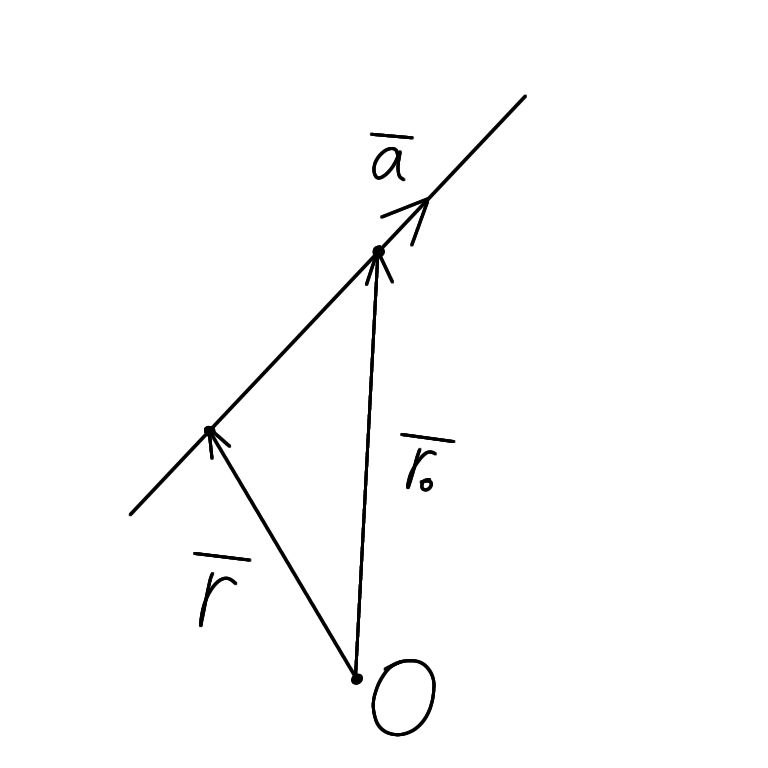
\includegraphics[width=0.84\linewidth]{images/1.1.jpeg}
\end{wrapfigure}

\tab\\
$\overline{a} \neq \overline{0}$ $-$ направляющий вектор\\

\underline{\textit{Векторное параметрическое уравнение прямой:}}
\[
\overline{r} = \overline{r_0} + \overline{a}t, t\in\R
\]
\[
\begin{pmatrix}
    x\\
    y\\
\end{pmatrix} = 
\begin{pmatrix}
    x_0\\
    y_0\\
\end{pmatrix} + 
\begin{pmatrix}
    a_x\\
    a_y\\
\end{pmatrix}t
\]
\tab\ \tab\\ \tab\\ \tab\\

\subsection{Общее уравнение прямой}

\begin{theorem}
    Любая прямая на плоскости может быть задана $\underline{\text{общим уравнением прямой}}$:
    \[
    Ax + By + C = 0, A^2 + B^2 > 0
    \]
\end{theorem}
\begin{proof}
    Точка $\overline{r}$ лежит на прямой тогда и только тогда, когда $\overline{r}$ - $\overline{r_0}$ и $\overline{a}$ $-$ коллинеарны, т.е.
    \[
    \begin{vmatrix}
        x - x_0 & y - y_0\\
        a_x & a_y\\
    \end{vmatrix} = 0
    \]
    \[
    \Longleftrightarrow
    \]
    \[
    a_y(x - x_0) - a_x(y-y_0) = 0
    \]
    \[
    \Longleftrightarrow
    \]
    \[
    a_y x - a_x y +(a_x y_0 - a_y x_0) = 0,
    \]
    \tab\\
    где $a_y$ = A, $- a_x$ = B, $a_x y_0 - a_y x_0$ = C
\end{proof}

\begin{corollary}
    В любой системе координат направляющий вектор прямой может быть выбран как (B, -A).
\end{corollary}

\begin{theorem}
    Если существует общее уравнение прямой, то оно задает прямую в любой системе координат.
\end{theorem}
\begin{proof}
    Рассмотрим точку ($x_0$, $y_0$), такую что
    \[
    Ax_0 + By_0 + C = 0
    \]
    Рассмотрим прямую, проходящую через точку ($x_0$, $y_0$), с направляющим вектором (В, -А). Подставив данные в векторное параметрическое уравнение прямой, получим искомое уравнение.
\end{proof}

\begin{theorem}
    Два уравнения задают одну прямую
    \[
    \begin{cases}
        A_1 x + B_1 y + C_1 = 0\\
        A_2 x + B_2 y + C_2 = 0\\
    \end{cases} \Longleftrightarrow \exists\lambda\neq 0 : A_1 = \lambda A_2, B_1 = \lambda B_2, C_1 = \lambda C_2
    \]
\end{theorem}
\begin{proof}
    \tab\\
    $\tab\Longleftarrow$\\
    Пусть $A_1 = \lambda A_2, B_1 = \lambda B_2, C_1 = \lambda C_2, \lambda\neq 0$. Подставим в общее уравнение прямой:
    \[
    A_1 x + B_1 y + C_1 = \lambda A_2 x + \lambda B_2 y + \lambda C_2 = \lambda(A_2 x + B_2 y + C_2) = 0,
    \]
    а т.к. $\lambda\neq 0$, получаем
    \[
    \begin{cases}
        A_1 x + B_1 y + C_1 = 0\\
        A_2 x + B_2 y + C_2 = 0\\
    \end{cases} - \text{одна прямая}
    \]

    $\tab\Longrightarrow$\\
    Т.к. заданные уравнения задают одну прямую, их направляющие векторы ($B_1$, -$A_1$) и ($B_2$, -$A_2$) $-$ коллинеарны $\Longrightarrow$ $\exists\lambda\neq 0$ : $A_1 = \lambda A_2, B_1 = \lambda B_2$, значит, чтобы уравнения были равносильны, необходимое условие: $C_1 = \lambda C_2$
\end{proof}

\subsection{Каноническое уравнение прямой}

Пусть задано 2 точки $\overline{r_1}$ и $\overline{r_2}$, значит направляющий вектор $\overline{a} = \overline{r_2} - \overline{r_1}$ $\Longrightarrow$
\[
\overline{r} = \overline{r_1} + t(\overline{r_2} - \overline{r_1})
\]
$-$ $\underline{\text{уравнение прямой через пару точек}}$.\\

Распишем координаты векторов.
\[
\begin{cases}
    x = x_0 + a_x t\\
    y = y_0 + a_y t\\
\end{cases} \Longrightarrow \dfrac{x - x_0}{a_x} = \dfrac{y - y_0}{a_y}
\]
Получили $\underline{\text{каноническое уравнение прямой}}$, причем при записи допускается, что $a_x$ или $a_y$ = 0. В таком случае задается прямая, параллельная одной из осей координат.\\

Аналогично для двух заданных точек $\overline{r_1}(x_1, y_1)$ и $\overline{r_2}(x_2, y_2)$:
\[
\dfrac{x - x_1}{x_2 - x_1} = \dfrac{y - y_1}{y_2 - y_1}
\]

\begin{corollary}
    Если задано каноническое уравнение прямой, то в знаменателях дробей стоят соответствующие координаты направляющего вектора. Это верно в любой системе координат.
\end{corollary}

\subsection{Уравнение прямой через нормальный вектор}

Если задать на прямой точку, ненулевой нормальный вектор $\overline{n}$ к этой прямой, то эта прямая задается однозначно.

\begin{wrapfigure}{l}{0.4\textwidth}
	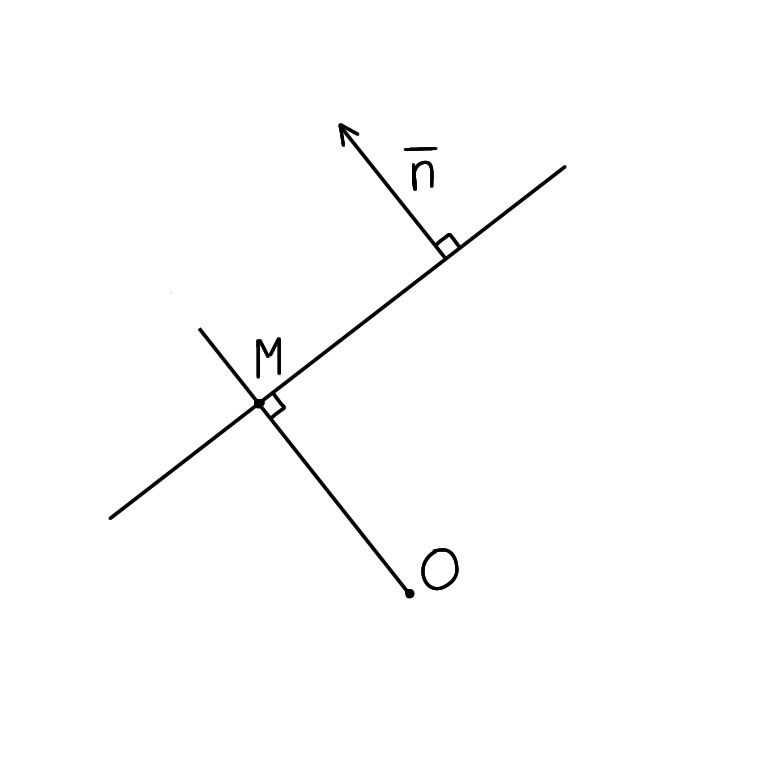
\includegraphics[width=0.84\linewidth]{images/1.2.jpeg}
\end{wrapfigure}

\tab\\

\[
(\overline{r} - \overline{r_0}, \overline{n}) = 0 \Longleftrightarrow (\overline{r}, \overline{n}) = (\overline{r_0}, \overline{n}) = d
\]

\[
\overline{r_M} = k\overline{n}, k = \dfrac{d}{(\overline{n}, \overline{n})}
\]

\[
\Longrightarrow \overline{r_M} = \dfrac{d}{(\overline{n}, \overline{n})}\overline{n}
\]

\tab\\
\textbf{В ОНБ.} 

\[
(\overline{r}, \overline{n}) = d, \text{где } \overline{r}(x, y), \overline{n}(n_x, n_y) \Longrightarrow n_x x + n_y y = d \Longrightarrow
\] если в ОНБ задано общее уравнение прямой, то вектор (А, В) $-$ один из нормальных векторов.

\subsection{Расстояние от точки до прямой}

\underline{В произвольной системе координат.}\\

Пусть заданы точка M : $\overline{r_1}$ и прямая l : ($\overline{r}$ - $\overline{r_0}$, $\overline{n}$) = 0.

\begin{wrapfigure}{l}{0.4\textwidth}
	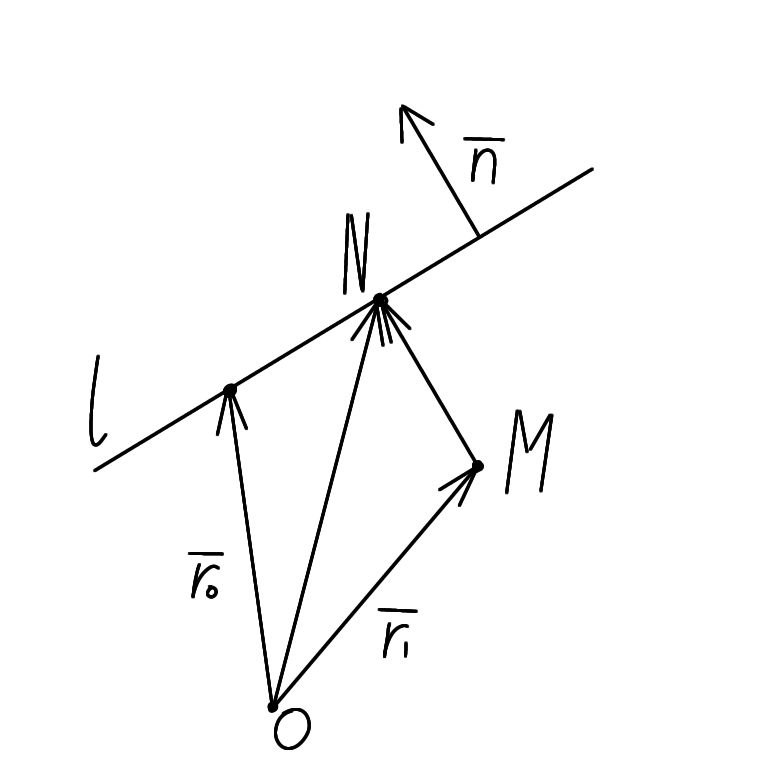
\includegraphics[width=0.84\linewidth]{images/1.3.jpeg}
\end{wrapfigure}

\tab\\

Тогда расстояние от точки М до прямой l \\
$\rho$ = |$\overline{MN}$|, $\overline{MN}$ = k$\overline{n}$

Мы знаем, что $\overline{ON}$ $-$ радиус-вектор точки, принадлежащей l $\Longrightarrow$ 

\[
(\overline{r_1} + k\overline{n} - \overline{r_0}, \overline{n}) = 0, k = \dfrac{(\overline{r_0} - \overline{r_1}, \overline{n})}{(\overline{n}, \overline{n})} \Longrightarrow
\]
\[
|\overline{MN}| = k\overline{n} = \dfrac{|(\overline{r_0} - \overline{r_1}, \overline{n})|}{|\overline{n}|} = |(\overline{r_0} - \overline{r_1}, \dfrac{\overline{n}}{|\overline{n}|})|
\]

\tab\\

\underline{В ОНБ.}\\

Пусть заданы точка М($x_1$, $y_1$) и прямая l : Ax + By + C = 0. Тогда в ОНБ расстояние от точки до прямой вычисляется как:
\[
\rho = \dfrac{|Ax_1 + By_1 + C|}{\sqrt{A^2 + B^2}}
\]

В любой системе координат прямая разбивает плоскость на 2 полуплоскости. Допустим, существует точка, лежащая вне прямой. Подставим эту точку в уравнение прямой, тогда в одной полуплоскости получим отрицательное значение, а в другой положительное.

\begin{wrapfigure}{l}{0.4\textwidth}
	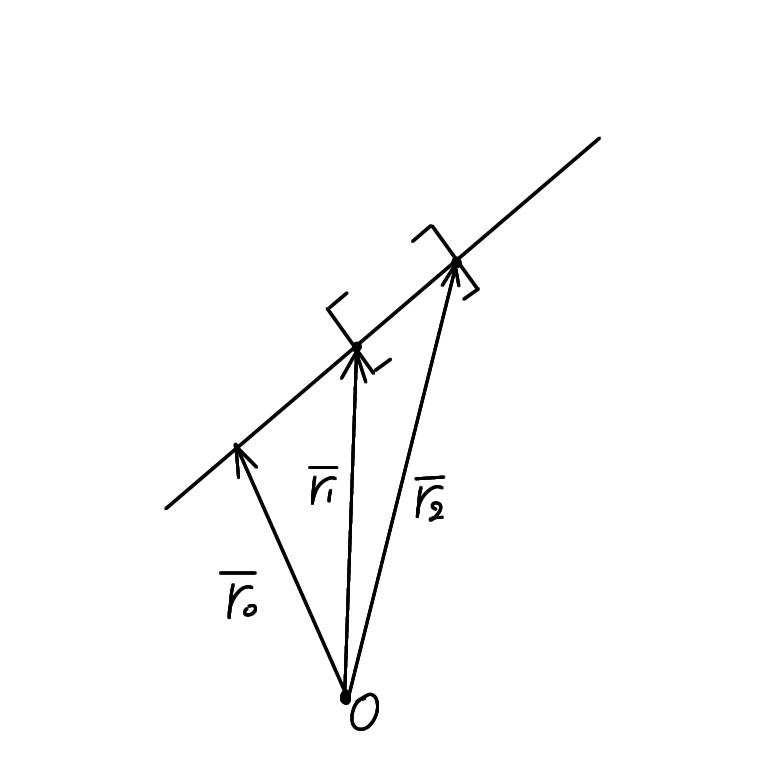
\includegraphics[width=0.84\linewidth]{images/1.4.jpeg}
\end{wrapfigure}

\tab\\

Чтобы задать отрезок на прямой, необходимо задать точки его концов
\[
\overline{r} = \overline{r_0} + t\overline{a}, t\in[t_1, t_2]
\]

\tab\\ \tab\\ \tab\\ \tab\\ \tab\\

\subsection{Пучок прямых}

\begin{definition}
    \textit{Пучок прямых} $-$ множество всех прямых, проходящих через заданную фиксированную точку.
\end{definition}

\begin{theorem}
    Пусть даны прямые
    \[
    \begin{cases}
        A_1 x + B_1 y + C_1 = 0\\
        A_2 x + B_2 y + C_2 = 0\\
    \end{cases} - \text{пересекающиеся} \Longrightarrow \text{пучок}.
    \] тогда
    \begin{enumerate}
        \item Для любой прямой пучка $\exists\alpha, \beta, \alpha^2 + \beta^2 > 0$ :
        \[
        \alpha(A_1 x + B_1 y + C_1) + \beta(A_2 x + B_2 y + C_2) = 0 - \text{уравнение этой прямой.}
        \]
        \item $\forall\alpha,\beta$, $\alpha^2 + \beta^2 > 0$:
        \[
        \alpha(A_1 x + B_1 y + C_1) + \beta(A_2 x + B_2 y + C_2) = 0 - \text{уравнение какой-то прямой из пучка.}
        \]
    \end{enumerate}
\end{theorem}
\begin{wrapfigure}{l}{0.4\textwidth}
    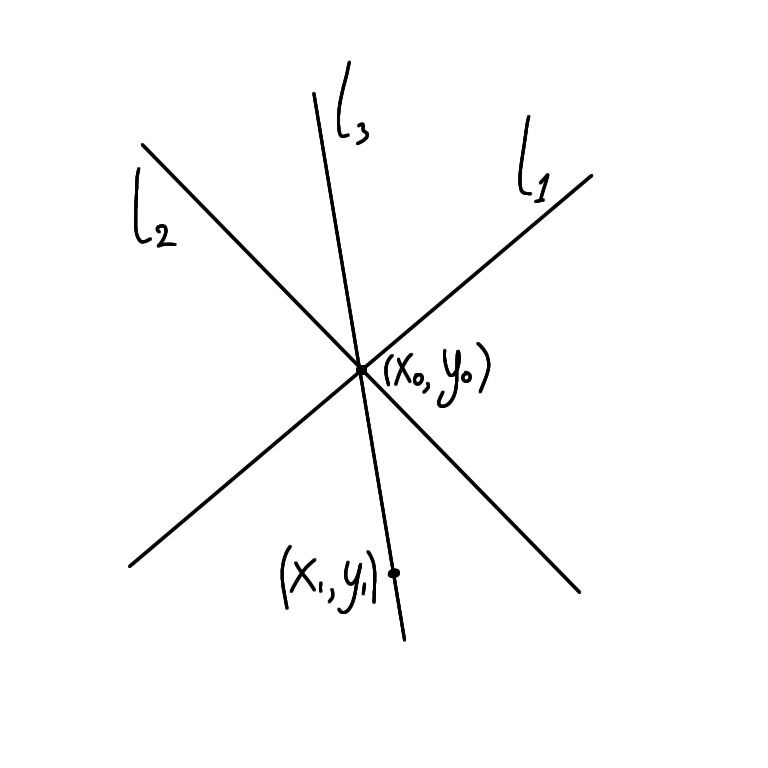
\includegraphics[width=0.84\linewidth]{images/1.5.jpeg}
\end{wrapfigure}

\tab\\

\begin{proof}
    Возьмем на $l_3$ точку ($x_1$, $y_1$), отличную от ($x_0$, $y_0$).
    Тогда
    \[
    (A_2 x_1 + B_2 y_1 + C_2)(A_1 x_1 + B_1 y_1 + C_1) - (A_1 x + B_1 y + C_1)(A_2 x + B_2 y + C_2) = 0,
    \]
    где $(A_2 x_1 + B_2 y_1 + C_2)$ = $\alpha$, $(-(A_1 x + B_1 y + C_1))$ = $\beta$ $\Longrightarrow$ $\alpha^2 + \beta^2 > 0$, т.к. ($x_1$, $y_1$) $\neq$ ($x_0$, $y_0$), но при этом ($x_1$, $y_1$) и ($x_0$, $y_0$) удовлетворяют этому уравнению.

    Осталось доказать, что полученное уравнение $-$ уравнение прямой, т.е. коэффициенты при x и y не могут одновременно равняться нулю, т.е.
    \[
    \left[
        \begin{gathered}
            \alpha A_1 + \beta A_2 \neq 0\\
            \alpha B_1 + \beta B_2 \neq 0\\
        \end{gathered}
    \right.
    \]
    Рассмотрим противное.
    $\begin{vmatrix}
        A_1 & A_2\\
        B_1 & B_2\\
    \end{vmatrix}$ $\neq$ 0, т.к. прямые различны $\Longrightarrow$ система имеет единственное решение при $\alpha$ = $\beta$ = 0 $\Longrightarrow$ противоречие
\end{proof}
\section{Плоскости в пространстве}

\subsection{Векторное параметрическое уравнение плоскости}

Пусть задана система координат O, $\overline{e_1}$, $\overline{e_2}$, $\overline{e_3}$.

\begin{wrapfigure}{l}{0.4\textwidth}
    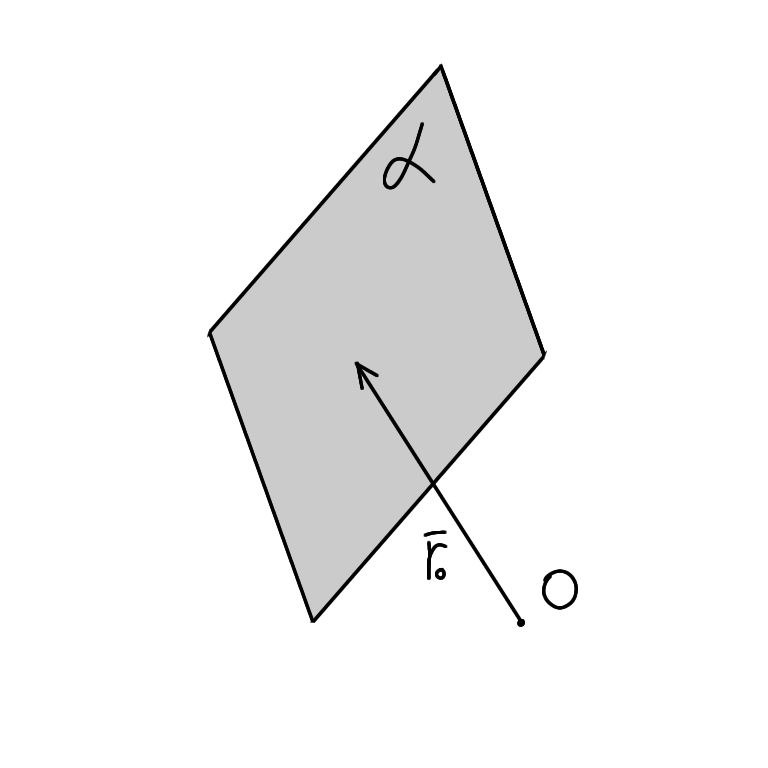
\includegraphics[width=0.84\linewidth]{images/2.1.jpeg}
\end{wrapfigure}

$\alpha$ $-$ плоскость в этой системе координат.\\

$\overline{p}$, $\overline{q}$ $-$ неколлинеарные и параллельные $\alpha$ вектора.\\

\underline{Векторное параметрическое уравнение плоскости}
\[
\overline{r} = \overline{r_0} + t_1\overline{p} + t_2\overline{q},\tab t_1, t_2\in\R
\]
\[
\begin{pmatrix}
    x\\
    y\\
    z\\
\end{pmatrix} = 
\begin{pmatrix}
    x_0\\
    y_0\\
    z_0\\
\end{pmatrix} + 
\begin{pmatrix}
    p_x\\
    p_y\\
    p_z\\
\end{pmatrix}t_1 + 
\begin{pmatrix}
    q_x\\
    q_y\\
    q_z\\
\end{pmatrix}t_2
\]
\tab\\

\subsection{Общее уравнение плоскости}

Заметим, что точка принадлежит плоскости $\Longleftrightarrow$ $\overline{r} - \overline{r_0}$, $\overline{p}$, $\overline{q}$ $-$ компланарны, т.е. ($\overline{r} - \overline{r_0}, \overline{p}, \overline{q}$) = 0 $\Longrightarrow$

\[
\begin{vmatrix}
    x - x_0 & y - y_0 & z - z_0\\
    p_x & p_y & p_z\\
    q_x & q_y & q_z\\
\end{vmatrix} = 0
\]
\[
\Longrightarrow 
\begin{vmatrix}
    p_y & p_z\\
    q_y & q_z\\
\end{vmatrix}(x - x_0) + 
\begin{vmatrix}
    p_x & p_z\\
    q_x & q_z\\
\end{vmatrix}(y - y_0) +
\begin{vmatrix}
    p_x & p_y\\
    q_x & q_y\\
\end{vmatrix}(z - z_0) = 0
\]

Таким образом, получили \underline{общее уравнение плоскости}

\[
\begin{cases}
    Ax + By + Cz + D = 0\\
    A^2 + B^2 + C^2 > 0 (\text{т.к. $\overline{p}$ и $\overline{q}$ - неколлинеарные})
\end{cases}
\]

\begin{theorem}
    Пусть в любой системе координат заданы общее уравнение плоскости Ax + By + Cz + D = 0 и вектор $\overline{a}(\alpha, \beta, \gamma)$ (возможен случай $\overline{a} = \overline{0}$).\\

    Тогда $\overline{a}$ параллелен плоскости $\Longleftrightarrow$ $A\alpha + B\beta + C\gamma$ = 0
\end{theorem}

\begin{proof}
    Пусть $\overline{r_0}(x_0, y_0, z_0)\in$плоскости $\Longrightarrow$ 
    \[
    Ax_0 + By_0 + Cz_0 + D = 0\eqno{(1)}
    \]

    $\overline{a}$ параллельно плоскости $\Longleftrightarrow$ $\overline{r_0} + \overline{a}$ принадлежит плоскости $\Longleftrightarrow$
    \[
    A(x_0 + \alpha) + B(y_0 + \beta) + C(z_0 + \gamma) + D = 0\eqno{(2)}
    \]

    Вычитая (1) из (2), получим $A\alpha + B\beta + C\gamma$ = 0
\end{proof}

\begin{corollary}
    Если задано уравнение вида Ax + By + Cz + D = 0 ($A^2 + B^2 + C^2 > 0$), то оно задает плоскость.
\end{corollary}
\begin{proof}
    Мы можем переписать уравнение в следующем виде

    \begin{itemize}
        \item При C $\neq$ 0:
        \[
        \begin{vmatrix}
            x + \dfrac{DA}{A^2 + B^2 + C^2} & y + \dfrac{DB}{A^2 + B^2 + C^2} & z + \dfrac{DC}{A^2 + B^2 + C^2}\\
            0 & -C & B\\
            C & 0 & -A\\
        \end{vmatrix} = 0
        \]
        где $\overline{p}$ = (0, -C, B) и $\overline{q}$ = (C, 0, -A) $-$ неколлинеарные вектора $\Longrightarrow$ уравнение задает плоскость.

        \item При С = 0:
        \[
        \begin{vmatrix}
            x + \dfrac{DA}{A^2 + B^2} & y + \dfrac{DB}{A^2 + B^2} & z + 0\\
            -B & A & 0\\
            0 & 0 & 1\\
        \end{vmatrix} = 0
        \]
        где $\overline{p}$ = (-B, A, 0) и $\overline{q}$ = (0, 0, 1) $-$ неколлинеарные вектора $\Longrightarrow$ уравнение задает плоскость.
    \end{itemize}
\end{proof}

\begin{theorem}
    Пусть плоскости П$_1$ и П$_2$ заданы следующими уравнениями
    \[
    A_1x + B_1y + C_1z + D_1 = 0\\
    A_2x + B_2y + C_2z + D_2 = 0\\
    \]
    Тогда П$_1$ параллельна П$_2$ $\Longleftrightarrow$ $\exists\lambda\neq 0 : A_1 = \lambda A_2$, $B_1 = \lambda B_2$, $C_1 = \lambda C_2$, $D_1 = \lambda D_2$
\end{theorem}

\subsection{Уравнение плоскости через 3 точки}

Пусть $\overline{r_1}(x_1, y_1, z_1)$, $\overline{r_2}(x_2, y_2, z_2)$, $\overline{r_3}(x_3, y_3, z_3)$ не лежат на одной прямой. Тогда
\[
\overline{r} = \overline{r_1} + t_1(\overline{r_2} - \overline{r_1}) + t_2(\overline{r_3} - \overline{r_1})
\]
\[
\begin{vmatrix}
    x - x_1 & y - y_1 & z - z_1\\
    x_2 - x_1 & y_2 - y_1 & z_2 - z_1\\
    x_3 - x_1 & y_3 - y_1 & z_3 - z_1\\
\end{vmatrix} = 0
\]
\clearpage
\subsection{Уравнение плоскости через нормальный вектор}

\begin{wrapfigure}{l}{0.4\textwidth}
    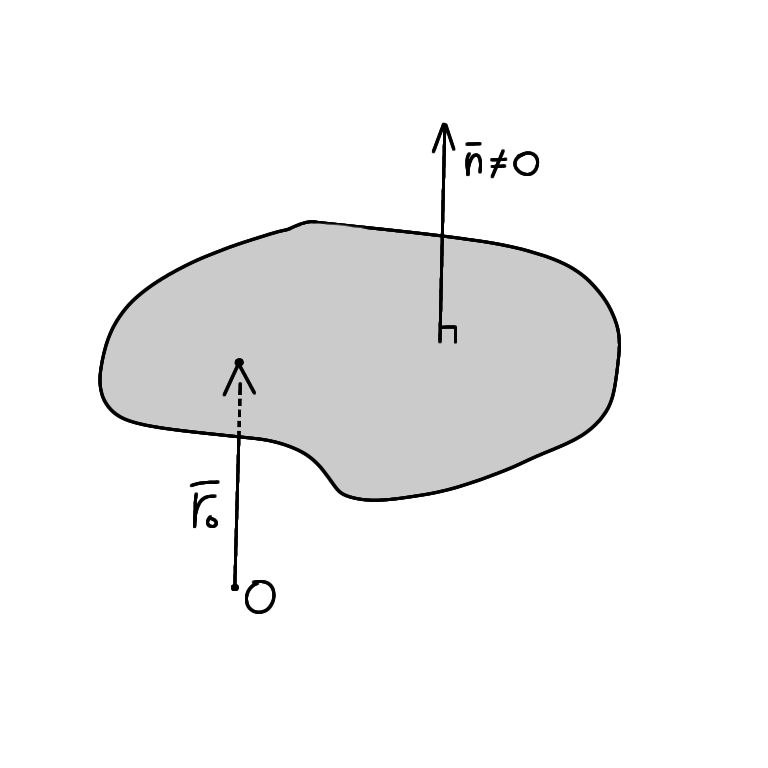
\includegraphics[width=0.84\linewidth]{images/2.2.jpeg}
\end{wrapfigure}

\tab\\

Пусть заданы точка $\overline{r_0}$, принадлежащая плоскости, и нормальный вектор $\overline{n}$. Тогда
\[
(\overline{r} - \overline{r_0}) = 0, \tab (\overline{r}, \overline{n}) = d
\]

В ОНБ один из способов задать нормалный вектор $\overline{n}$ = (A, B, C).

\tab\\ \tab\\ \tab\\ \tab\\
\subsection{Расстояние от точки до плоскости}

\underline{В произвольной системе координат.}\\

Пусть заданы точка $M_0$($\overline{r_1}$) и плоскость ($\overline{r} - \overline{r_0}$, $\overline{n}$) = 0. Тогда расстояние от $M_0$ до плоскости
\[
\rho = \dfrac{|(\overline{r_1} - \overline{r_0}, \overline{n})|}{|\overline{n}|}
\]

\underline{В ОНБ.}\\

\[
\overline{n}(A, B, C), M(x_1, y_1, z_1), Ax + By + Cz + D = 0 \Longrightarrow
\]
\[
\rho = \dfrac{|Ax_1 + By_1 + Cz_1 + D|}{\sqrt{A^2 + B^2 + C^2}}
\]
\subsection{Пучок плоскостей}

\begin{definition}
    \textit{Пучок плоскостей} $-$ множество плоскостей, проходящих через одну прямую.
\end{definition}

\begin{definition}
    \textit{Связка плоскостей} $-$ множество плоскостей, проходящих через одну точку.
\end{definition}
\clearpage
\section{Прямые в пространстве}

\subsection{Способы задания прямой в пространстве}

\underline{Каноническое уравнение прямой}\\

\begin{wrapfigure}{l}{0.3\textwidth}
    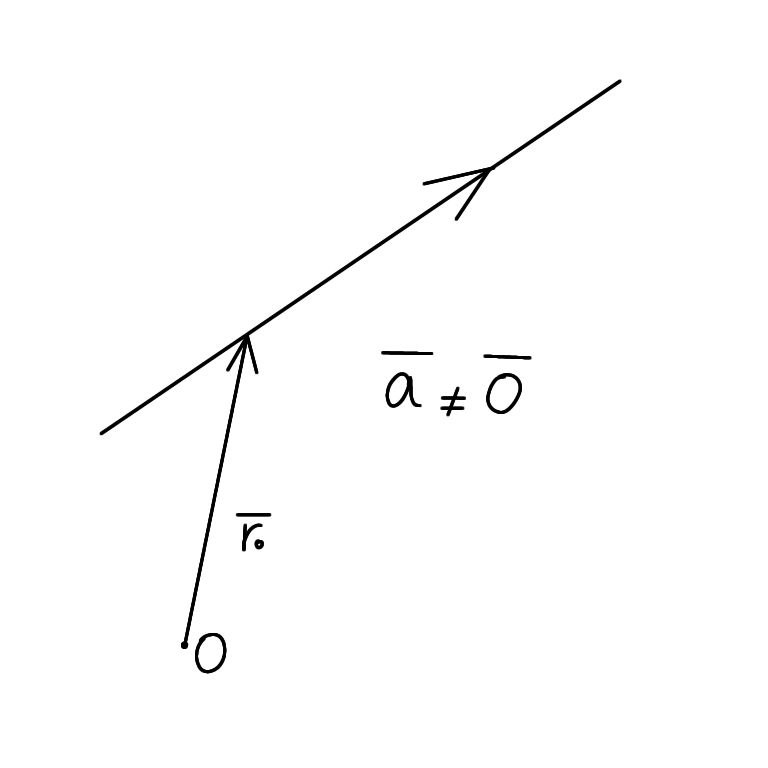
\includegraphics[width=0.84\linewidth]{images/3.1.jpeg}
\end{wrapfigure}

\tab\\

\[
\begin{cases}
    \overline{r} = \overline{r_0} + \overline{a}t\\
    x = x_0 + a_xt\\
    y = y_0 + a_yt\\
    z = z_0 + a_zt\\
\end{cases} 
\]
\[
\Longrightarrow \tab \dfrac{x - x_0}{a_x} = \dfrac{y - y_0}{a_y} = \dfrac{z - z_0}{a_z}
\]
\tab\\
\underline{Через пару точек $\overline{r_1}$ и $\overline{r_2}$}\\

\[
\overline{r} = \overline{r_1} + t(\overline{r_2} - \overline{r_1})
\]
\[
\Longleftrightarrow
\]
\[
\dfrac{x - x_1}{x_2 - x_1} = \dfrac{y - y_1}{y_2 - y_1} = \dfrac{z - z_1}{z_2 - z_1}
\]

\underline{Через направляющий вектор}\\

\[
[\overline{r} - \overline{r_0}, \overline{a}] = \overline{0}\\
\]
\[
[\overline{r}, \overline{a}] = \overline{d}
\]

\underline{Через две плоскости}\\

Пусть заданы две плоскости П$_1$ и П$_2$, тогда прямая $-$ пересечение этих плоскостей.

\subsection{Углы между прямыми и плоскостями}

\begin{definition}
    Углом между плоскостями ($\overline{r} - \overline{r_{01}}, \overline{n_1}$) = 0 и ($\overline{r} - \overline{r_{02}}, \overline{n_2}$) = 0 называется угол между их нормальными векторами $\overline{n_1}$ и $\overline{n_2}$.
\end{definition}

\begin{definition}
    Углом между плоскостью ($\overline{r} - \overline{r_{0}}, \overline{n}$) = 0 и прямой $\overline{r}$ = $\overline{r_0} + t\overline{a}$ называется угол $\dfrac{\pi}{2} - \alpha$, где $\alpha$ - угол между векторами $\overline{n}$ и $\overline{a}$.
\end{definition}

\subsection{Расстояния между точками, прямыми и плоскостями в пространстве}

\underline{Расстояние от точки до прямой в пространстве}\\

\begin{wrapfigure}{l}{0.3\textwidth}
    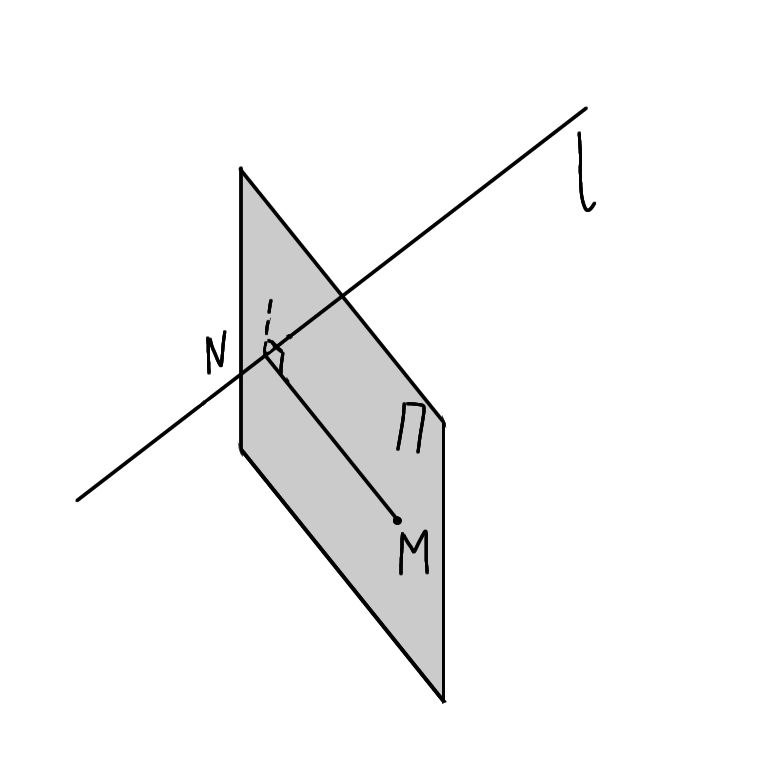
\includegraphics[width=0.84\linewidth]{images/3.2.jpeg}
\end{wrapfigure}
\tab\\

    1 способ. Проведем плоскость П, которая проходит через точку М перпендикулярно прямой l. Тогда
    \[
    \rho = \rho(M, N)
    \]

    \tab\\ \tab\\ \tab\\ \tab\\ \tab\\

\begin{wrapfigure}{l}{0.3\textwidth}
    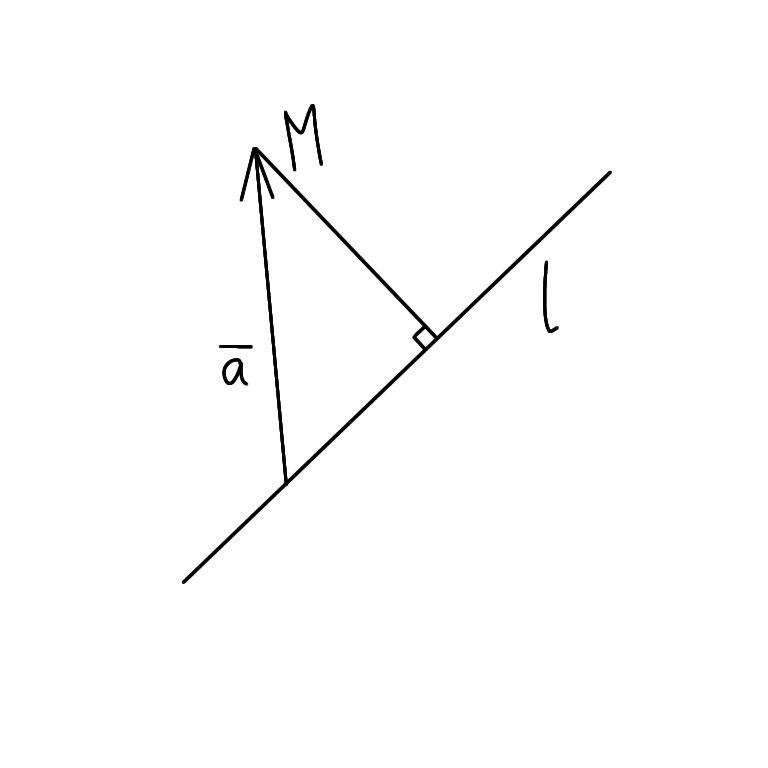
\includegraphics[width=0.84\linewidth]{images/3.3.jpeg}
\end{wrapfigure}
\tab\\

    2 способ. Спроецируем $\overline{a}$ на прямую l и найдем ортогональную составляющую $-$ искомое расстояние.

    \tab\\ \tab\\ \tab\\ \tab\\ \tab\\ \tab\\ \tab\\

\begin{wrapfigure}{l}{0.3\textwidth}
    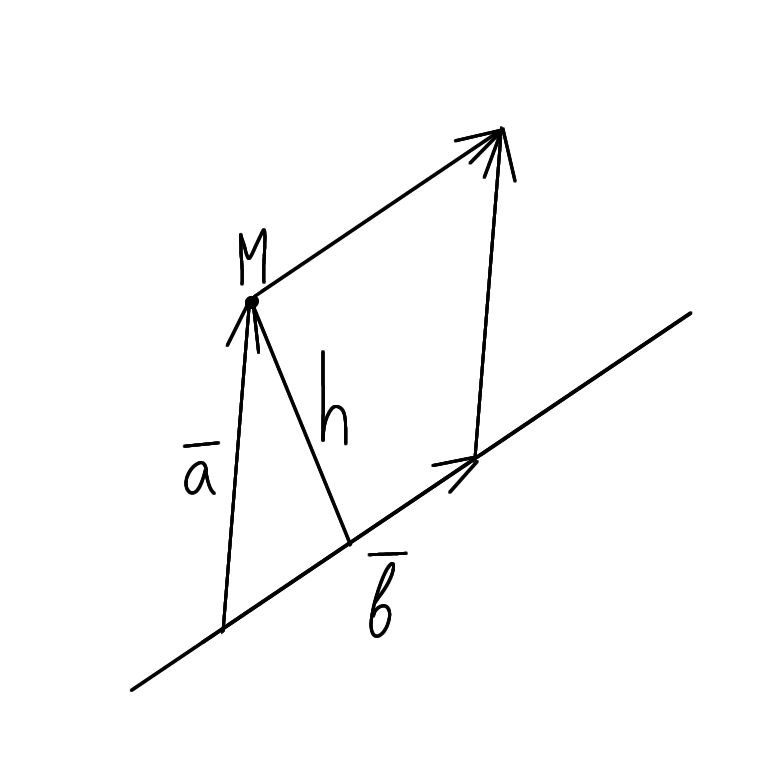
\includegraphics[width=0.84\linewidth]{images/3.4.jpeg}
\end{wrapfigure}
\tab\\

    3 способ. \[
    \rho = \dfrac{S\mkern-2mu{\rotatebox{-60}{\(\lozenge\)}}}{|\overline{b}|} = \dfrac{|[\overline{a}, \overline{b}]|}{|\overline{b}|}
    \]

    \tab\\ \tab\\ \tab\\ \tab\\ \tab\\
\underline{Расстояние между прямыми в пространстве}\\

Пусть заданы две прямые $l_1$ и $l_2$.\\

Если $l_1$ || $l_2$, то расстояние от любой точки $l_1$ до $l_2$ $-$ искомое.\\

Если $l_1$ и $l_2$ $-$ скрещивающиеся (возможно пересечение), то\\

\begin{wrapfigure}{l}{0.3\textwidth}
    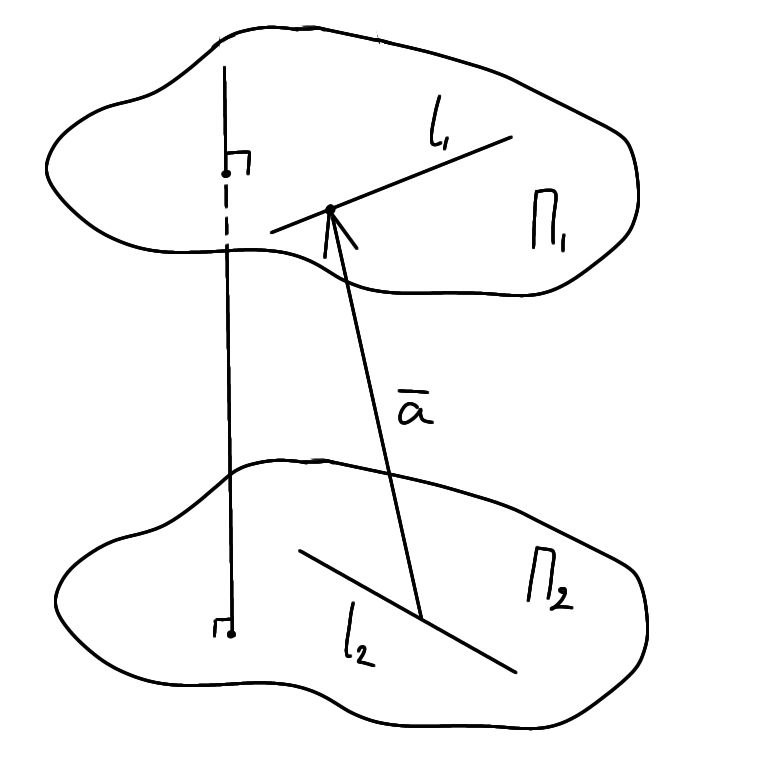
\includegraphics[width=0.84\linewidth]{images/3.6.jpeg}
\end{wrapfigure}

\tab\\

1 способ. Проведем плоскость через $l_1$ параллельно $l_2$  и посчитаем расстояние от точки на $l_2$  до плоскости.\\

2 способ. Проведем через прямые параллельные плоскости, а к ним проведем общий перпендикуляр, тогда искомое расстояние $-$ скалярная проекция $\overline{a}$ на него.\\

3 способ. \[
\rho = \dfrac{|(\overline{a}, \overline{b}, \overline{c})|}{|[\overline{a}, \overline{b}]|}
\]
\section{Алгебраические линии и поверхности}

В пространстве рассмотрим уравнения вида
\[
A_1 x^{\alpha_1}y^{\beta_1}z^{\gamma_1} + A_2 x^{\alpha_2}y^{\beta_2}z^{\gamma_2} + ... + A_k x^{\alpha_k}y^{\beta_k}z^{\gamma_k} = 0,\tab \alpha_i, \beta_i, \gamma_i \in \Z \geq 0
\]

\begin{definition}
    \textit{Степень уравнения}, или \textit{порядок алгебраической поверхности} $-$
    \[
    T = \underset{i=1..k}{max}(\alpha_i + \beta_i + \gamma_i)
    \]

    Аналогично на плоскости задается алгебраическая линия порядка T = $\underset{i=1..k}{max}(\alpha_i + \beta_i)$
\end{definition}

\begin{theorem}
    Алгебраическая поверхность(линия) порядка p в любой системе координат может быть задана уравнением порядка p.
\end{theorem}
\begin{proof}
    \[
    \begin{cases}
        x = a_{11}x' + a_{12}y' + a_{13}z'\\
        y = a_{21}x' + a_{22}y' + a_{23}z'\\
        z = a_{31}x' + a_{32}y' + a_{33}z'\\
    \end{cases}
    \]
    Подставив полученные координаты в уравнение, получим, что максимальная степень m такая, что порядок не увеличится.

    Заметим также, что если порядок уменьшится, то при обратной замене он должен увеличиться, значит получим противоречие $\Longrightarrow$ порядок не изменился.
\end{proof}

\begin{lemma}
    Пусть существует алгебраическая поверхность(линия) порядка n. Тогда прямая и алгебраическая поверхность(линия) могут иметь 0, 1, ..., n или бесконечно много общих точек.
\end{lemma}














\section{Линии второго порядка}

\begin{definition}
    \textit{Линиями второго порядка} на плоскоти называются алгебраические линии следующего вида
    \[
    \begin{cases}
        Ax^2 + 2Bxy + Cy^2 + 2Dx + 2Ey + F = 0\\
        A^2 + B^2 + C^2 > 0\\f
    \end{cases}
    \]
\end{definition}
\textbf{В ПДСК:} $\Delta$ = 
$\begin{vmatrix}
    A & B\\
    B & C\\
\end{vmatrix}
$ $-$ неизменная величина при изменении системы координат.\\

\begin{proposition}
    Существует ПДСК, в которой тип кривой второго порядка может быть записан одним из 9 способов (канонических уравнений):
    \begin{itemize}
        \item $\Delta$ > 0 - эллиптический тип
        \begin{enumerate}
            \item $\dfrac{x^2}{a^2}$ + $\dfrac{y^2}{b^2}$ = 1, $a\geq b>0$ $-$ эллипс
            \item $\dfrac{x^2}{a^2}$ + $\dfrac{y^2}{b^2}$ = 0 $-$ пара мнимых пересекающихся прямых
            \item $\dfrac{x^2}{a^2}$ + $\dfrac{y^2}{b^2}$ = -1 $-$ мнимый эллипс
        \end{enumerate}
        \item $\Delta$ < 0 - гиперболический тип
        \begin{enumerate}
            \item $\dfrac{x^2}{a^2}$ - $\dfrac{y^2}{b^2}$ = 1, $a\geq b>0$ $-$ гипербола
            \item $\dfrac{x^2}{a^2}$ - $\dfrac{y^2}{b^2}$ = 0 $-$ пара пересекающихся прямых
        \end{enumerate}
        \item $\Delta$ = 0 - параболический тип
        \begin{enumerate}
            \item $y^2$ = 2px, p > 0 $-$ парабола
            \item $y^2$ = $a^2$, a > 0 $-$ пара параллельных прямых
            \item $y^2$ = 0 $-$ пара совпадающих прямых
            \item $y^2$ = -$a^2$, a > 0 $-$ пара мнимых параллельных прямых
        \end{enumerate}
    \end{itemize}
\end{proposition}

\subsection{Поворот системы координат}

$Ax^2 + 2Bxy + Cy^2 + 2Dx + 2Ey + F = 0$\\

Будем считать, что $B\geq 0$, $A\geq C$. Обнулим коэффициент при ху.\\

Существует угол $\alpha$, на котороый можно повернуть систему координат так, чтобы коэффициент В стал равен 0.
\[
\begin{cases}
    x = cos \alpha \cdot x' - sin \alpha \cdot y'\\
    y = sin \alpha \cdot x' + cos \alpha \cdot y'
\end{cases} \Longrightarrow
\]
\[
A'x'^2 + 2B'x'y' + C'y'^2 + 2D'x' + 2E'y' + F' = 0
\]
\[
A' = A cos^2\alpha + 2B sin \alpha \cdot cos \alpha + C sin^2\alpha
\]
\[
2B' = -2A sin \alpha \cdot cos \alpha + 2B cos^2\alpha - 2B sin^2\alpha + 2C sin \alpha \cdot cos \alpha
\]
\[
C' = A sin^2\alpha - 2B sin \alpha \cdot cos \alpha + C cos^2\alpha\\
\]
При замене координат A' + C' = A + C, $\Delta = \begin{vmatrix}
    A' & B'\\
    B' & C'\\
\end{vmatrix} = \begin{vmatrix}
    A & B\\
    B & C\\
\end{vmatrix}$\\

Покажем, что существует угол $\alpha$ такой что, при повороте системы координат на него, В = 0.
Т.к. $2B' = -2A sin \alpha \cdot cos \alpha + 2B cos^2\alpha - 2B sin^2\alpha + 2C sin \alpha \cdot cos \alpha$
\[
tg \alpha = \dfrac{2B}{A - C}
\]
\begin{enumerate}
    \item Если А = С, то в качестве угла $\alpha$ можно взять угол $\dfrac{\pi}{4}$
    \item Если А $\neq$ C
    \[
    tg^2\alpha + \dfrac{A - C}{B}tg \alpha - 1 = 0 \tab - \text{всегда имеет хотя бы одно решение}
    \]
    $\Longrightarrow$ всегда можно сделать поворот системы координат $\Longrightarrow$
    \[
    \begin{cases}
        B' = 0\\
        A' + C' = A + C\\
        \Delta = const\\
    \end{cases}
    \]
\end{enumerate}

\section{Эллипс}

\begin{wrapfigure}{l}{0.5\textwidth}
    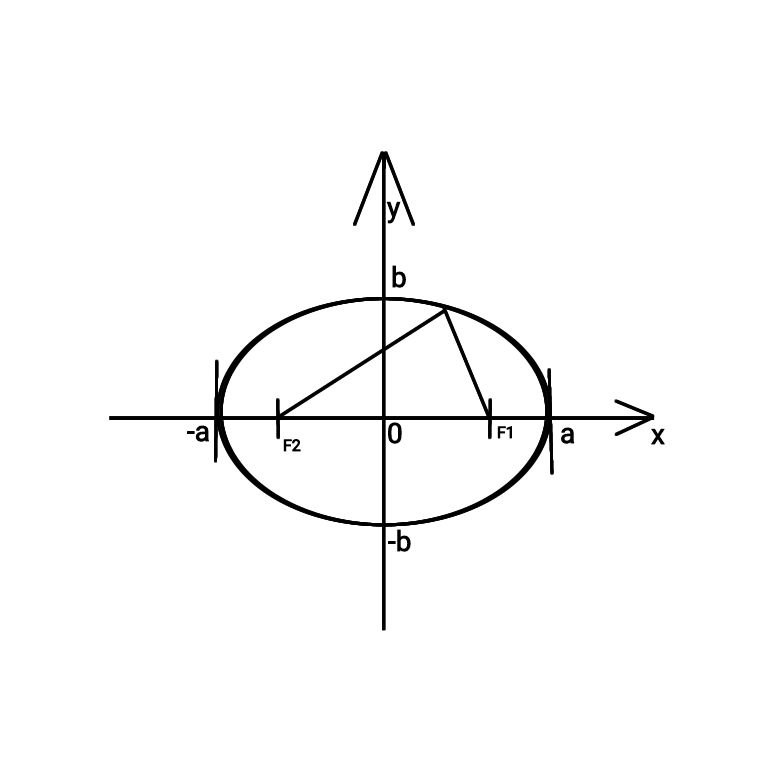
\includegraphics[width=0.84\linewidth]{images/эллипс1.jpeg}
\end{wrapfigure}

\tab\\

Каноническое уравнение эллипса
\[
\dfrac{x^2}{a^2} + \dfrac{y^2}{b^2} = 1, \tab a\geq b > 0
\]

\underline{Свойства множества точек эллипса:}
\begin{enumerate}
    \item Непустое
    \item Ограниченное
    \item Обладает осевой и центральной симметрией
\end{enumerate}

\clearpage
\subsection{Свойства фокусов и эксцентрисетета эллипса}

Рассмотрим a $\neq$ b. Эллипс пересекает оси координат в вершинах эллипса  $-$ $\pm$a, $\pm$b\\
    
Пусть c = $\sqrt{a^2 - b^2}$, тогда фокусы эллипса $-$ точки $F_1$(c, 0), $F_2$(-c, 0).\\
    
Эксцентриситет $\varepsilon$ = $\dfrac{c}{a}$ = $\dfrac{\sqrt{a^2 - b^2}}{a}$, $\varepsilon\in[0, 1)$, причем если $\varepsilon$ = 0, то этот эллипс - окружность.\\

\subsection{Расстояние от точки на эллипсе до фокусов и директрис}

Из теоремы Пифагора
\[
\rho(F_1, A) = (x_0 - c)^2 + y_0^2 = x_0^2 - 2x_0c + c^2 - \dfrac{x_0^2b^2}{a^2} + b^2 = x_0^2 \dfrac{a^2 - b^2}{a^2} - 2x_0\varepsilon a + a^2 = (x_0\varepsilon - a)^2
\]
Аналогично находится $\rho(F_2, A)$, таким образом
\[
\rho(F_1, A) = a - x_0\varepsilon
\]
\[
\rho(F_2, A) = x_0\varepsilon + a
\]

\begin{theorem}
    $\rho(F_1, A)$ + $\rho(F_2, A)$ = 2a
\end{theorem}
\begin{proof}
    $\rho(F_1, A) + \rho(F_2, A)$ = $a - x_0\varepsilon + x_0\varepsilon + a$ = 2a
\end{proof}

\begin{wrapfigure}{l}{0.45\textwidth}
    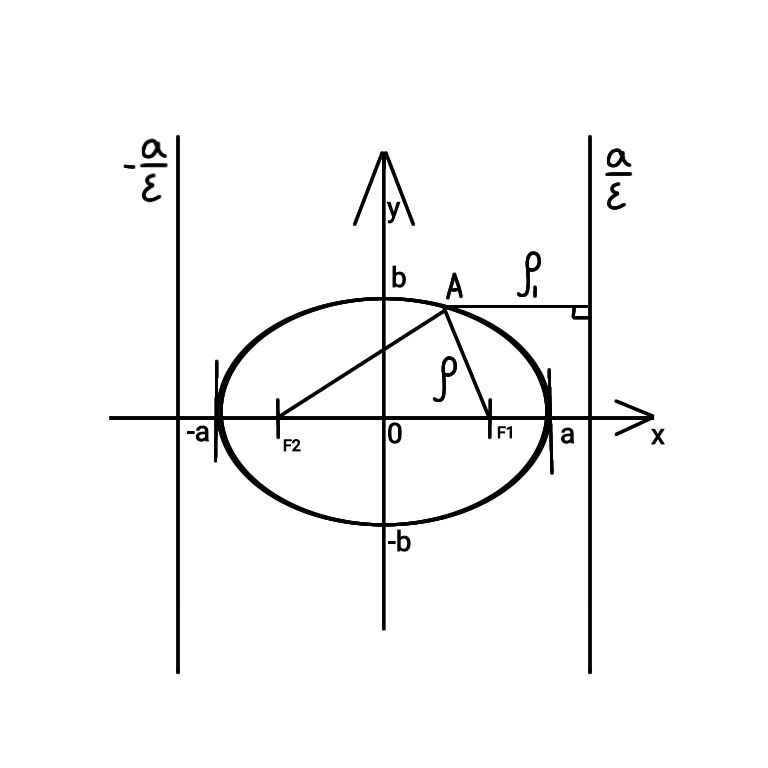
\includegraphics[width=1.0\linewidth]{images/эллипс2.jpeg}
\end{wrapfigure}

\tab\\

\begin{definition}
    Директрисы эллипса задаются уравнением x = $\pm\dfrac{a}{\varepsilon}$
\end{definition}

У окружности директрис $\underline{\text{нет}}$.\\

\begin{proposition}
    Расстояние от точки на эллипсе до фокуса $\rho(F_1, A)$ относится к расстоянию от этой точки до ближайшей директрисы $\rho_1$ как эксцентрисетет.
    \[
    \dfrac{\rho(F_1, A)}{\rho_1} = \varepsilon
    \]
\end{proposition}
\begin{proof}
    Это следует из того, что $\rho(F_1, A) = a - x_0\varepsilon$ и $\rho_1 = \dfrac{a}{\varepsilon} - x_0$
\end{proof}

\clearpage

\subsection{Касательные к эллипсу}

\begin{proposition}
    Пусть эллипс задан уравнением $\dfrac{x^2}{a^2} + \dfrac{y^2}{b^2} = 1$, точка A($x_0$, $y_0$) лежит на эллипсе. Тогда уравнение касательной к эллипсу, проведенной через точку А имеет вид
    \[
    \dfrac{xx_0}{a^2} + \dfrac{yy_0}{b^2} = 1
    \]
\end{proposition}
\begin{proof}
    \begin{enumerate}
        \item Касательные вертикальны $\Longrightarrow$ x = $\pm$a $\longrightarrow$ $x_0$ = $\pm$a, $y_0$ = 0 $\Longrightarrow$ верно.
        \item Касательные не вертикальны $\Longrightarrow$
        \[
        y - y_0 = y'(x_0)(x - x_0)\eqno{(*)}
        \]
        Продифференцируем уравнение эллипса по х:
        \[
        \dfrac{2x}{a^2} + \dfrac{2yy'}{b^2} = 0 \tab\Longrightarrow\tab y'(x_0) = - \dfrac{x_0}{y_0}\cdot\dfrac{b^2}{a^2}
        \]
        Подставим в уравнение (*)
        \[
        y - y_0 = - \dfrac{x_0}{y_0}\cdot\dfrac{b^2}{a^2}\cdot(x - x_0)
        \]
        Домножив на $\dfrac{y_0}{b^2}$, получим
        \[
        \dfrac{x^2}{a^2} + \dfrac{y^2}{b^2} = \dfrac{x_0^2}{a^2} + \dfrac{y_0^2}{b^2} = 1, (\text{т.к точка А лежит на эллипсе)}
        \]
    \end{enumerate}
\end{proof}

\subsection{Оптическое свойство эллипса}
\begin{wrapfigure}{l}{0.45\textwidth}
    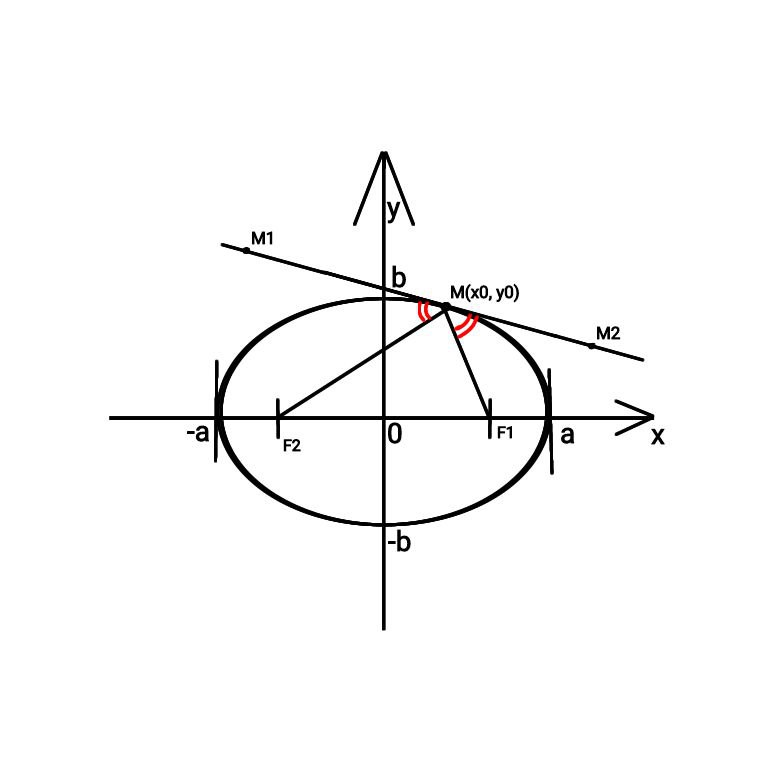
\includegraphics[width=1.0\linewidth]{images/эллипс3.jpeg}
\end{wrapfigure}

\tab\\

\begin{theorem}
    Пусть M($x_0$, $y_0$) - точка на эллипсе, $M_1M_2$ - касательная, проходящая через эту точку. Тогда, углы $F_1MM_2$ и $F_2MM_1$ равны.
\end{theorem}
\begin{proof}
    Достаточно доказать, что
    \[
    \angle(\overline{n}, \overline{F_1M}) = \angle(\overline{n}, \overline{F_2M})
    \]
    \[
    \begin{cases}
        \overline{F_1M}(x_0 + c, y_0)\\
        \overline{F_2M}(x_0 - c, y_0)\\
        \overline{n}(\dfrac{x_0}{a^2}, \dfrac{y_0}{b^2})
    \end{cases} \Longrightarrow
    \]
    \clearpage
    Докажем, что $\dfrac{(\overline{F_1M}, \overline{n})}{|\overline{F_1M}|\cdot|\overline{n}|}$ = $\dfrac{(\overline{F_2M}, \overline{n})}{|\overline{F_2M}|\cdot|\overline{n}|}$
    \[
    \dfrac{(x_0 - c)\dfrac{x_0}{a^2} + \dfrac{y_0^2}{b^2}}{a - \varepsilon x_0} = \dfrac{(x_0 + c)\dfrac{x_0}{a^2} + \dfrac{y_0^2}{b^2}}{a + \varepsilon x_0} \tab\Longrightarrow\tab\text{верно}
    \]
\end{proof}

\section{Гипербола}

\begin{wrapfigure}{l}{0.55\textwidth}
    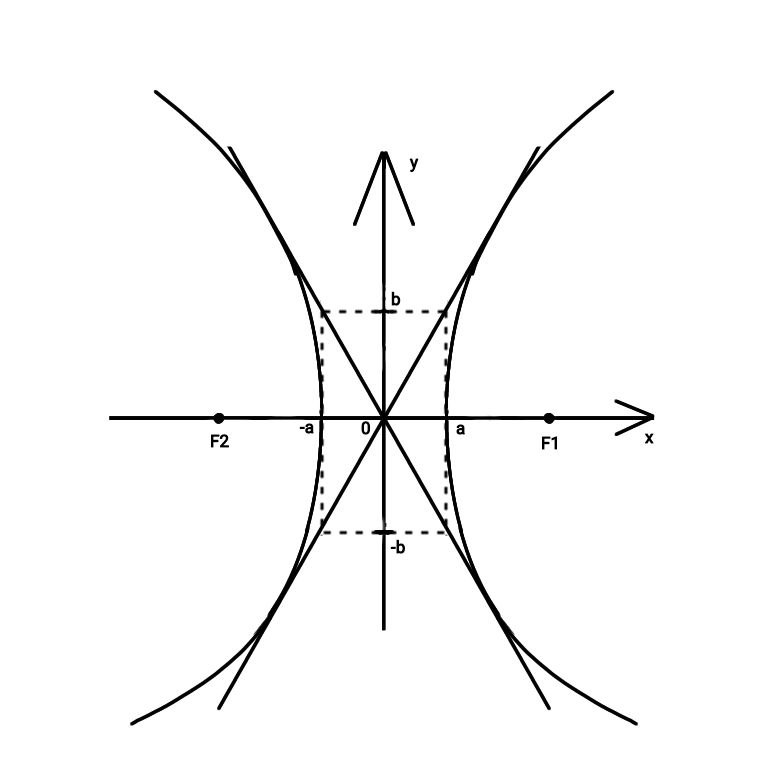
\includegraphics[width=1.0\linewidth]{images/гипербола1.jpeg}
\end{wrapfigure}

\tab\\

Каноническое уравнение гиперболы
\[
\dfrac{x^2}{a^2} - \dfrac{y^2}{b^2} = 1, \tab a, b \neq 0
\]

\underline{Свойства множества точек гиперболы:}
\begin{enumerate}
    \item Непустое
    \item Неограниченное
    \item Обладает осевой и центральной симметрией
\end{enumerate}

\tab\\ \tab\\ \tab\\ \tab\\ \tab\\ \tab\\ \tab\\ \tab\\ \tab\\

\subsection{Свойства фокусов и эксцентрисетета гиперболы}

Из уравнения гиперболы y = $\pm\dfrac{b}{a}\sqrt{x^2 - a^2}$.\\

Пусть x > 0, тогда y = $\dfrac{b}{a}\sqrt{x^2 - a^2}$ $\Longrightarrow$ множество точек гиперболы находится ниже прямой y = $\dfrac{b}{a}x$. Аналогично при x < 0 множество точек гиперболы находится ниже прямой y = -$\dfrac{b}{a}x$.\\

Пусть c = $\sqrt{a^2 + b^2}$, тогда фокусы эллипса $-$ точки $F_1$(c, 0), $F_2$(-c, 0).\\
    
Эксцентриситет $\varepsilon$ = $\dfrac{c}{a}$ = $\dfrac{\sqrt{a^2 + b^2}}{a}$, $\varepsilon > 1$.\\

\subsection{Расстояние от точки на гиперболе до фокусов и директрис}

\begin{wrapfigure}{l}{0.6\textwidth}
    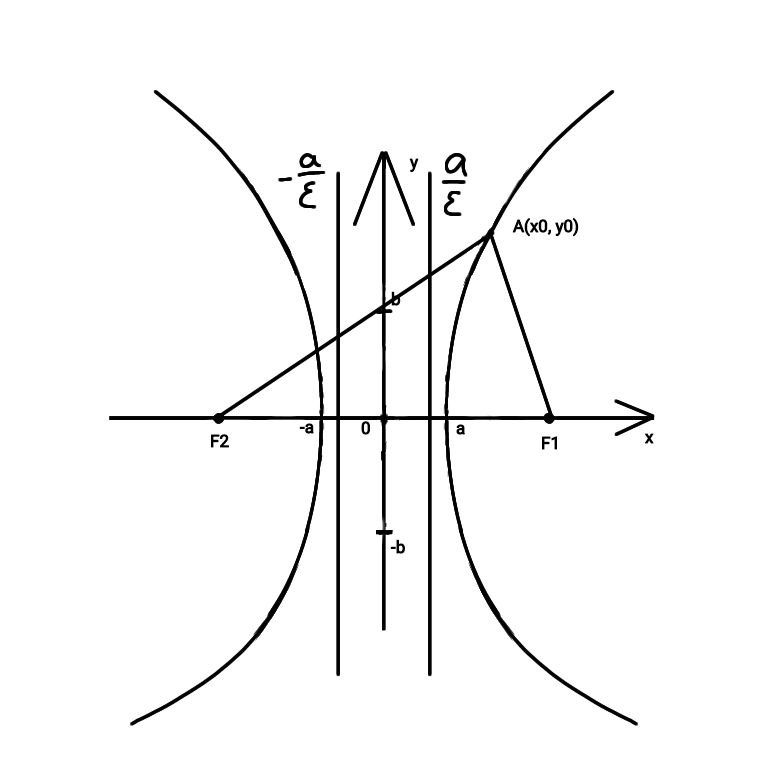
\includegraphics[width=0.8\linewidth]{images/гипербола2.jpeg}
\end{wrapfigure}

\tab\\

Пусть А($x_0$, $y_0)$ - точка на гиперболе. Тогда расстояния от нее до фокусов равны

\[
\rho(F_1, A) = |a - \varepsilon x_0|
\tab\\
\rho(F_2, A) = |a + \varepsilon x_0|
\]

Знак, с которым раскрываются модули, зависит от того, на какой ветви гиперболы находится точка А
\begin{enumerate}
    \item x > 0 $\Longrightarrow$
    $\begin{cases}
        \rho(F_1, A) = \varepsilon x_0 - a\\
        \rho(F_2, A) = a + \varepsilon x_0
    \end{cases}$
    \item x < 0 $\Longrightarrow$
    $\begin{cases}
        \rho(F_1, A) = a - \varepsilon x_0\\
        \rho(F_2, A) = -a - \varepsilon x_0
    \end{cases}$
\end{enumerate}

\begin{proposition}
    $|\rho(F_1, A)$ - $\rho(F_2, A)|$ = 2a
\end{proposition}
\tab\\
\begin{definition}
    Директрисы гиперболы задаются уравнением x = $\pm\dfrac{a}{\varepsilon}$
\end{definition}

\begin{proposition}
    Расстояние от точки на гиперболе до фокуса $\rho(F_1, A)$ относится к расстоянию от этой точки до ближайшей директрисы $\rho_1$ как эксцентрисетет.
    \[
    \dfrac{\rho(F_1, A)}{\rho_1} = \varepsilon
    \]
\end{proposition}
\clearpage

\subsection{Касательные к гиперболе}

Пусть гипербола задана уравнением $\dfrac{x^2}{a^2} - \dfrac{y^2}{b^2} = 1$, точка A($x_0$, $y_0$) лежит на гиперболе. Тогда уравнение касательной к гиперболе, проведенной через точку А имеет вид
    \[
    \dfrac{xx_0}{a^2} - \dfrac{yy_0}{b^2} = 1
    \]
\subsection{Оптическое свойство гиперболы}

\begin{wrapfigure}{l}{0.55\textwidth}
    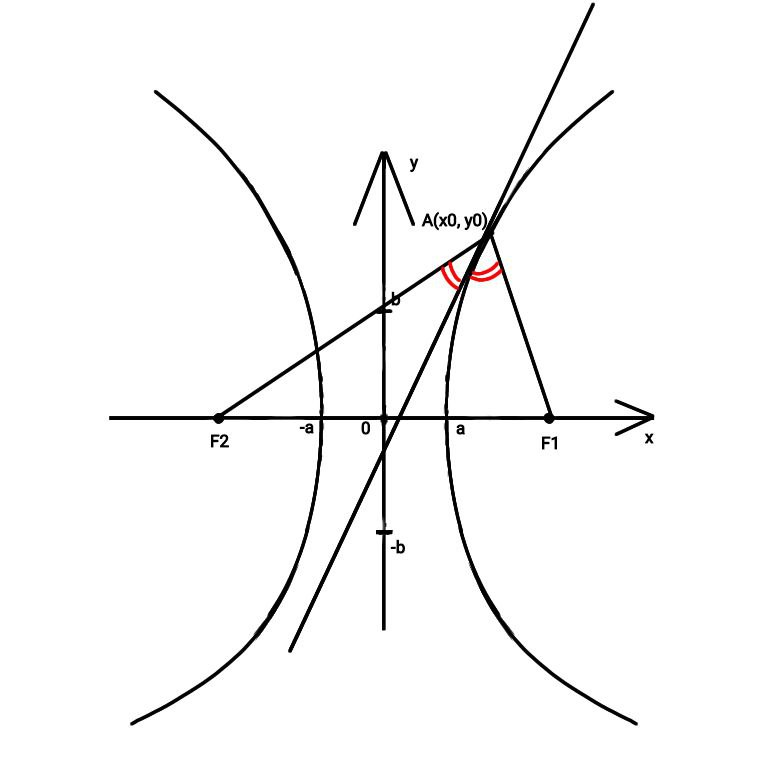
\includegraphics[width=.8\linewidth]{images/гипербола3.jpeg}
\end{wrapfigure}
\tab\\ 
\begin{theorem}
    Пусть A($x_0$, $y_0$) - точка на гиперболе, через которую провели касательную. Тогда, углы, образованные этой касательной и фокальными радиусами точки, равны.
\end{theorem}
\tab\\ \tab\\ \tab\\ \tab\\ \tab\\ \tab\\ \tab\\ \tab\\ \tab\\ 
\section{Парабола}

\begin{wrapfigure}{l}{0.6\textwidth}
    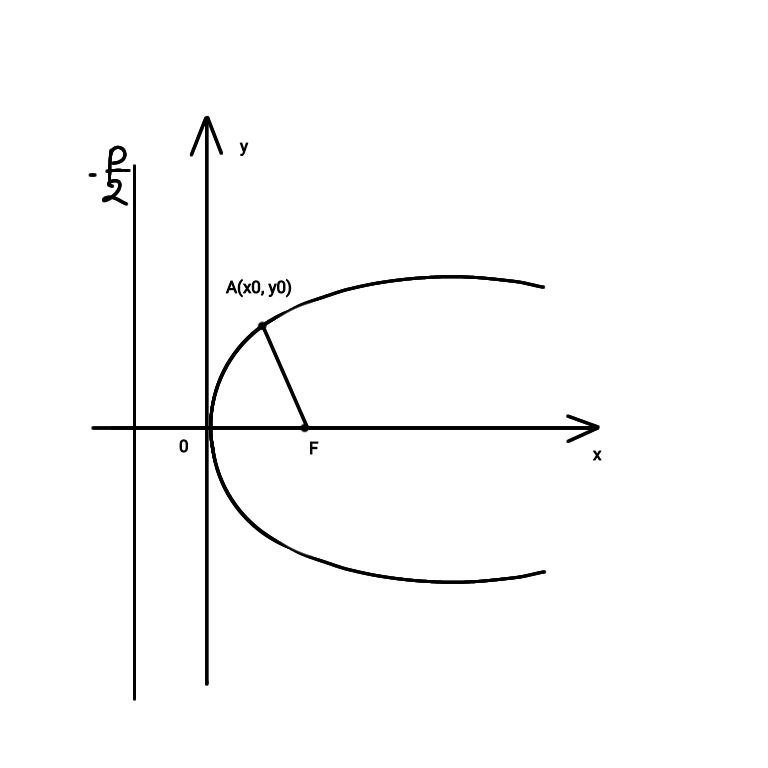
\includegraphics[width=.8\linewidth]{images/парабола1.jpeg}
\end{wrapfigure}

\tab\\ 

Каноническое уравнение параболы
\[
y^2 = 2px, p > 0
\]

\underline{Свойства множества точек эллипса:}
\begin{enumerate}
    \item Непустое
    \item Неограниченное
    \item Симметричное относительно одной из осей
\end{enumerate}
\clearpage

\subsection{Свойства фокуса и эксцентрисетета параболы}

Эксцентрисетет параболы равен 1, фокус один и находится в точке с координатами ($\dfrac{p}{2}$, 0).

\subsection{Расстояние от точки на параболы до фокуса и директрисы}

Пусть А($x_0$, $y_0)$ - точка на параболе. Тогда расстояние от нее до фокуса равно

\[
\rho(F, A) = x_0 + \dfrac{p}{2}
\]

\begin{definition}
    Директриса параболы задается уравнением x = -$\dfrac{p}{2}$
\end{definition}

Расстояние от точки А($x_0$, $y_0)$ на параболе до директрисы равно $x_0 + \dfrac{p}{2}$

\subsection{Касательные к параболе}

Пусть парабола задана уравнением $y^2 = 2px$, точка A($x_0$, $y_0$) лежит на параболе. Тогда уравнение касательной к параболе, проведенной через точку А имеет вид
    \[
    yy_0 = p(x + x_0)
    \]
    
\subsection{Оптическое свойство параболы}

\begin{wrapfigure}{l}{0.5\textwidth}
    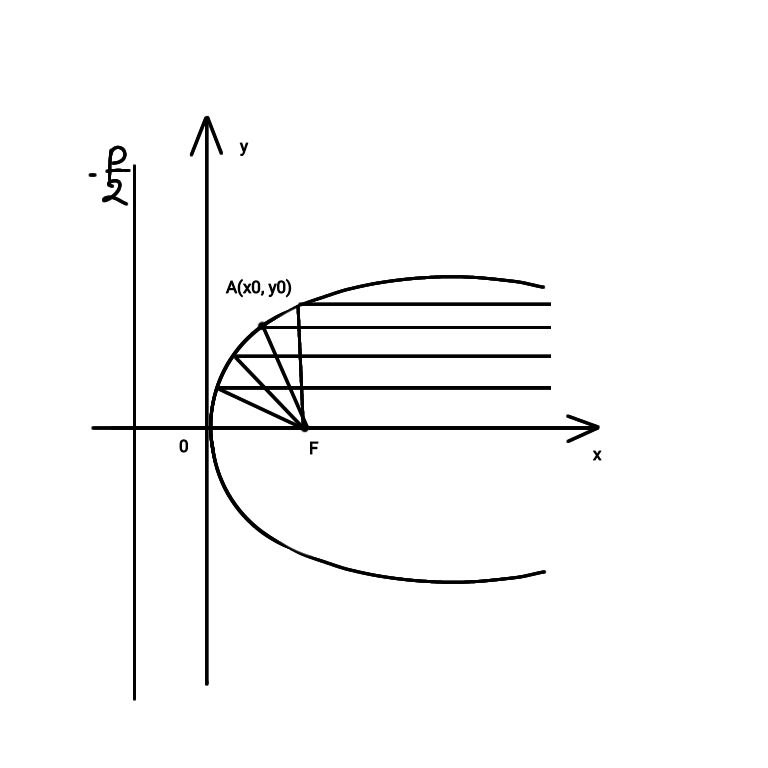
\includegraphics[width=1.0\linewidth]{images/парабола2.jpeg}
\end{wrapfigure}

\tab\\
\begin{theorem}
    Параллельные лучи приходят в фокус параболы и проходят одинаковые расстояния.
\end{theorem}



















\section{Поверхности второго порядка}

Пусть задана плоскость, а в ней линия, заданная функцией f(x, z). Начнем вращать линия вокруг оси Oz. Каждая точка на линии описывает окружность радиусом |x|, при этом z сохраняется, но изменяется координата по y, т.е. |x| = $\sqrt{x^2 + y^2}$ $\Longrightarrow$
\[
f(\sqrt{x^2 + y^2}, z)\cdot f(-\sqrt{x^2 + y^2}, z) = 0 - \underline{\text{уравнение поверхности вращения}}
\]

Рассмотрим линию в пространстве и вектор $\overline{a}\neq\overline{0}$. Назовем линию \textit{направляющей} и проведем через каждую точку, лежащую на ней, \textit{образующие}, параллельные $\overline{a}$. Таким образом, получим \underline{цилиндрическую поверхность}.\\

\underline{Коническая поверхность} образована прямыми, проходящими через все точки направляющей кривой и точку, лежащую вне этой кривой.\\

\begin{definition}
    \textit{Поверхность второго порядка} задается следующим образом
    \[
    \begin{cases}
        A_1x^2 + A_2y^2 + A_3z^2 + 2A_4xy + 2A_5xz + 2A_6yz + 2A_7x + 2A_8y + 2A_9z + A_{10} = 0\\
        A_1^2 + A_2^2 + A_3^2 + A_4^2 + A_5^2 + A_6^2 > 0
    \end{cases}
    \]
\end{definition}

Всего 17 типов поверхностей второго порядка.\\

Прямая и поверхность второго порядка имеют либо 0, либо 1, либо 2 общие точки, либо прямая целиком принадлежит поверхности.\\

\begin{definition}
    Прямая, целиком лежащая на поверхности, называется \textit{прямолинейной образующей} этой поверхности.
\end{definition}

\subsection{Эллипсоид}

\begin{wrapfigure}{l}{0.5\textwidth}
    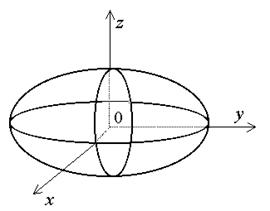
\includegraphics[width=1.0\linewidth]{images/эллипсоид.jpg}
\end{wrapfigure}

\tab\\

\underline{Уравнение:}
\[
\dfrac{x^2}{a^2} + \dfrac{y^2}{b^2} + \dfrac{z^2}{c^2} = 1 \tab a, b, c > 0
\]

\underline{Основные сечения:}
\begin{itemize}
    \item Эллипсы
\end{itemize}

\underline{Свойства:}
\begin{itemize}
    \item Центральная и осевая симметрии
    \item Ограниченность
    \item Если 2 коэффициента равны, то это эллипсоид вращения
    \item Если все коэффициенты совпадают, то это сфера
    \item Нет прямолинейных образующих
\end{itemize}

\subsection{Эллиптический параболоид}
\begin{wrapfigure}{l}{0.5\textwidth}
    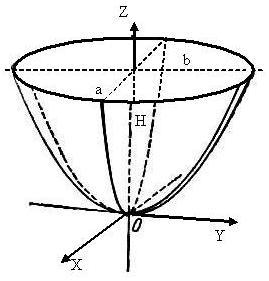
\includegraphics[width=1.0\linewidth]{images/эллиптический параболоид.JPG}
\end{wrapfigure}

\tab\\

\underline{Уравнение:}
\[
\dfrac{x^2}{a^2} + \dfrac{y^2}{b^2} = 2z \tab a, b > 0
\]

\underline{Основные сечения:}
\begin{itemize}
    \item Эллипс - 1 сечение
    \item Параболы - 2 сечения
\end{itemize}

\underline{Свойства:}
\begin{itemize}
    \item Неограниченность
    \item Осевая симметрия
    \item Если a = b, то это параболоид вращения
    \item Нет прямолинейных образующих
\end{itemize}
\tab\\ \tab\\ \tab\\ \tab\\
\subsection{Гиперболический параболоид}

\begin{wrapfigure}{l}{0.5\textwidth}
    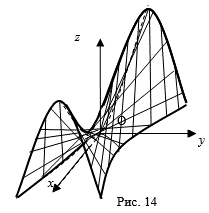
\includegraphics[width=0.7\linewidth]{images/гиперболический параболоид.png}
\end{wrapfigure}

\tab\\

\underline{Уравнение:}
\[
\dfrac{x^2}{a^2} - \dfrac{y^2}{b^2} = 2z \tab a, b > 0
\]

\underline{Основные сечения:}
\begin{itemize}
    \item Параболы - 2 сечения
    \item Гипербола - 1 сечение
\end{itemize}

\clearpage
\underline{Свойства:}
\begin{itemize}
    \item  Неограниченность
    \item Осевая симметрия
    \item Через каждую точку можно провести 2 прямолинейные образующие
\end{itemize}


\subsection{Однополостный гиперболоид}

\begin{wrapfigure}{l}{0.5\textwidth}
    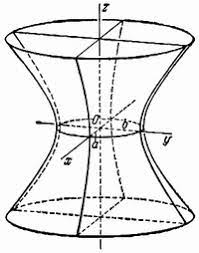
\includegraphics[width=0.7\linewidth]{images/однополостный гиперболоид.jpeg}
\end{wrapfigure}

\underline{Уравнение:}
\[
\dfrac{x^2}{a^2} + \dfrac{y^2}{b^2} - \dfrac{z^2}{c^2} = 1 \tab a, b, c > 0
\]

\underline{Основные сечения:}
\begin{itemize}
    \item Эллипс - 1 сечение
    \item Гиперболы - 2 сечения
\end{itemize}

\underline{Свойства:}
\begin{itemize}
    \item Неограниченность
    \item Центральная и осевая симметрии
    \item Если 2 коэффициента равны, то это гиперболоид вращения
    \item Через каждую точку можно провести 2 прямолинейные образующие
\end{itemize}

\tab\\ \tab\\
\subsection{Конус}

\begin{wrapfigure}{l}{0.5\textwidth}
    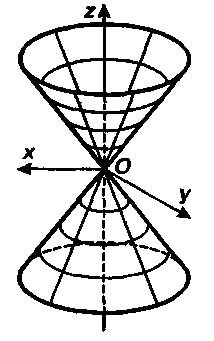
\includegraphics[width=0.5\linewidth]{images/конус.jpg}
\end{wrapfigure}

\tab\\

\underline{Уравнение:}
\[
\dfrac{x^2}{a^2} + \dfrac{y^2}{b^2} - \dfrac{z^2}{c^2} = 0 \tab a, b, c > 0
\]

\underline{Основные сечения:}
\begin{itemize}
    \item Эллипс
    \item Парабола
    \item Гипербола
\end{itemize}
\clearpage
\underline{Свойства:}
\begin{itemize}
    \item Неограниченность
    \item Центральная и осевая симметрии
    \item Если 2 коэффициента равны, то это гиперболоид вращения
    \item Через каждую точку можно провести 1 прямолинейную образующую, через вершину проходят все линейные образующие
\end{itemize}

\subsection{Двуполостный гиперболоид}

\begin{wrapfigure}{l}{0.5\textwidth}
    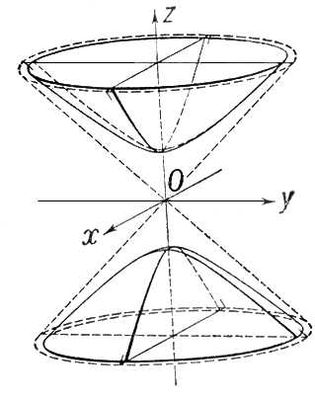
\includegraphics[width=.7\linewidth]{images/двуполостный гиперболоид.jpg}
\end{wrapfigure}

\tab\\ 

\underline{Уравнение:}
\[
-\dfrac{x^2}{a^2} - \dfrac{y^2}{b^2} + \dfrac{z^2}{c^2} = 1 \tab a, b, c > 0
\]

\underline{Основные сечения:}
\begin{itemize}
    \item Эллипс - 1 сечение
    \item Гипербола - 2 сечения
\end{itemize}

\underline{Свойства:}
\begin{itemize}
    \item Неограниченность
    \item Центральная и осевая симметрии
    \item Нет прямолинейных образующих
\end{itemize}

\tab\\ \tab\\ \tab\\
\subsection{Параболический цилиндр}

\begin{wrapfigure}{l}{0.5\textwidth}
    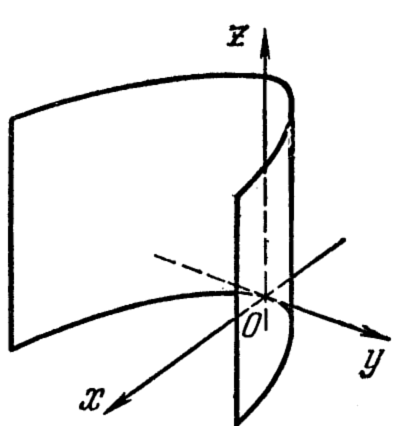
\includegraphics[width=.5\linewidth]{images/параболический цилиндр.png}
\end{wrapfigure}

\tab\\

\underline{Уравнение:}
\[
y^2 = 2px
\]
\clearpage
\subsection{Гиперболический цилиндр}

\begin{wrapfigure}{l}{0.5\textwidth}
    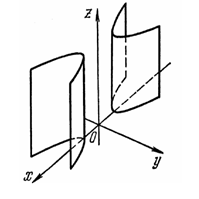
\includegraphics[width=.5\linewidth]{images/гиперболический цилиндр.png}
\end{wrapfigure}

\tab\\

\underline{Уравнение:}
\[
\dfrac{x^2}{a^2} - \dfrac{y^2}{b^2} = 1
\]

\tab\\ \tab\\ \tab\\ \tab\\ 
\subsection{Эллиптический цилиндр}

\begin{wrapfigure}{l}{0.5\textwidth}
    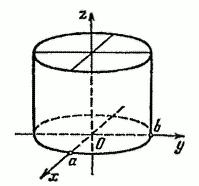
\includegraphics[width=.5\linewidth]{images/эллиптический цилиндр.jpeg}
\end{wrapfigure}

\tab\\

\underline{Уравнение:}
\[
\dfrac{x^2}{a^2} + \dfrac{y^2}{b^2} = 1
\]

